\documentclass[oneside, 12pt, a4paper]{book}

\errorcontextlines=5 % Adjust the number to show more or fewer lines

\makeatletter
\def\input@path{{./templates/}}
\usepackage{thesis_uc3m}
\graphicspath{{./figures} {./templates/figures}}
\makeatother

\title{Applications of Autonomous Drones for Non-Terrestrial Networks in Remote Areas}
\author{Andrés Navarro Pedregal}
\degree{Data Science and Engineering and Telecommunication Technologies Engineering}
\graduationyear{2024~--~2025}
\supervisor{José Alberto Hernández Gutierrez}
\placeandyear{Leganés, 2025}

\hypersetup{
  pdfauthor=Andres Navarro Pedregal,
  pdftitle=Final Thesis | Andres Navarro Pedregal | Data Science and Engineering,
  pdfsubject=Final Thesis,
  pdfkeywords={Final Thesis, Andres Navarro Pedregal, Data Science and Engineering},
}

\addbibresource{./bibliography.bib} % load the bibliography file

\loadglsentries{acronyms} % load the acronyms file

\begin{document}

% \setcounter{tocdepth}{0} % Show only parts and chapters in the table of contents

\frontmatter
\maketitle

\blankpage%
\chapter*{Abstract}

this is an abstract

\textbf{Keywords:} keyword1, keyword2, keyword3

\blankpage%

\chapter*{Acknowledgments}
\begingroup
\let\clearpage\relax % This temporarily disables \clearpage so the Agradecimientos chapter is on the same page

Thanks

\chapter*{Agradecimientos}

Gracias

\endgroup

\blankpage%

\renewcommand{\contentsname}{Table of Contents}
\tableofcontents

\blankpage%

\listoffigures

\blankpage%

\listoftables

\blankpage%

\printglossary[type=\acronymtype,style=long]

\blankpage%

\mainmatter%

\oldpart{Introduction} % So there is no new page before the first chapter, thus the page number is correct

\chapter{Motivation}\label{ch:motivation}

\todo{write this chapter}

% As of 2024-10-20, this part has been completed and reviewed by Andres

\chapter{Statement of the problem}\label{ch:statement_of_problem}

Current research in the domain of \gls{ntn} primarily focuses on the development of satellite constellations in \gls{geo} and \gls{leo} \autocite{non_terrestial_networks_trends}. Despite the fact that these satellites offer significant potential, their high costs and limited customizability render them impractical for many research groups and individual researchers. Moreover, the complexity of launching and maintaining satellites in orbit presents a significant barrier to entry for many interested parties.

This work seeks to address the gap by developing a comprehensive, open-source, and cost-effective solution for the deployment of \glspl{uav} in remote environments to study and research \glspl{ntn}. Moreover, this solutions seeks to open the door to a new area of research in the domain of \gls{ntn}, low altitude \gls{uav}-based networks, and to provide a platform for researchers and individuals to explore other potential applications of \glspl{uav} in remote areas.

Given the broad nature of this problem, the scope of this thesis will be narrowed to a specific environment and use case, as outlined below:

\begin{itemize}
  \item \textbf{Environment:} The modeled environment will be a remote area with minimal infrastructure, such as a forest, desert, or mountain. Specifically, the case study will involve an esplanade—a flat area devoid of significant obstacles like buildings or trees—allowing the \gls{uav} to operate without the risk of collision. Moreover, \gls{4g} or \gls{5g} connectivity will be assumed to be available, enabling the \gls{uav} to communicate with a control station.

  \item \textbf{Atmospheric Conditions:} The selected environment will feature a clear sky, with minimal electromagnetic interference from other sources such as \glspl{uav} or aircrafts. Additionally, the conditions will approximate \gls{stp} of \SI{15}{\degreeCelsius} and \SI{1013}{\hecto\pascal}.

  \item \textbf{Operational Parameters:} The \gls{uav} operations will be confined to \gls{vlos} and an altitude below \SI{120}{\metre} and the \gls{mtow} of the \gls{uav} will not exceed \SI{25}{\kilogram}, ensuring compliance with current aviation regulations in Spain and most countries.

  \item \textbf{Hardware:} The \gls{uav} will be constructed using commercially available, off-the-shelf components to ensure affordability and ease of replication for other research groups and individuals.
\end{itemize}

% Local Variables:
% jinx-local-words: "customizability mtow ntn terrestial uav"
% End:

\chapter{Objectives}
\label{ch:objectives}

The primary aim of this thesis is to develop an open-source, modular, and customizable drone capable of operating in remote areas. This drone will possess autonomous flight capabilities and the ability to communicate with a ground station. Furthermore, it will allow for remote control and can be programmed to perform specific tasks, making it suitable for various applications, including reconnaissance, surveillance, agriculture, and humanitarian aid.

In addition, a software platform will be developed to enable the programming of the drone for reconnaissance tasks. This software will be designed to support multiple drones, facilitating the creation of a coordinated swarm for reconnaissance operations.

The drone's design will emphasize ease of assembly, disassembly, repair, and maintenance. It will be cost-effective and user-friendly, allowing for straightforward customization and modification.

To achieve these objectives, the following specific aims will be pursued:

\begin{itemize}
  \item The design must be modular and customizable, enabling easy modifications to adapt the drone for different applications.

  \item The components utilized in the drone should be off-the-shelf and readily available, facilitating straightforward assembly and repairs.

  \item The drone must be capable of autonomous flight to enable operations in remote areas where manual control is challenging.

  \item The design will incorporate the latest advancements in drone technology, ensuring competitiveness with other market offerings.

  \item The drone must be capable of communicating with a ground station to facilitate remote control.

  \item The system should be programmable to perform specific tasks, such as reconnaissance of designated areas and monitoring of particular parameters.

  \item The software platform must support multiple drones, allowing for the deployment of a coordinated swarm to conduct reconnaissance tasks effectively.
\end{itemize}

\chapter{Document Structure}

\chapter{Methodological Framework}\label{ch:methodology_approach}

The methodological framework employed in this thesis is grounded in the V-model as established by the \gls{incose} \autocite{INCOSE2015} for project development. The V-model offers a rigorous and structured method that ensures all project facets are considered, facilitating timely and budget-compliant completion. This is achieved through a comprehensive development process, enabling clear validation and verification of initial requirements at every stage.

The methodology is segmented into seven key components which can be summarized as follows:

\begin{enumerate}
  \item \textbf{Identification of User Requirements}: A detailed analysis of the problem statement is conducted to identify the primary issues and potential solutions. Moreover, the user requirements are defined to ensure that the proposed solution aligns with the objectives of the project.

  \item \textbf{System Design}: The system architecture is developed based on the user requirements, ensuring that the proposed solution is feasible and aligns with the project's objectives. This phase includes a detailed overview of the system components and their interconnections. Requirements are formulated to satisfy the previously defined solution requirements. This phase includes a high-level overview of the components of the proposed solution, the justification for their selection, and the interconnections among them.

  \item \textbf{Component Design}: Building upon the high-level architecture of the solution, a more detailed approach is outlined for each component, taking into account their specific power and data transmission needs. This culminates in a comprehensive architecture of the solution. Furthermore, a detailed overview of the components is provided, including the rationale for their selection and the interconnections among them.

  \item \textbf{Implementation}: The proposed solution is implemented and manufactured utilizing available tools while simultaneously integrating the necessary electrical components. This phase includes a detailed description of the implementation process, including the tools and materials used, as well as the integration of electrical components. The development of software and hardware components is also detailed.

  \item \textbf{Component Testing}: The functionality of each component is verified in a standalone mode, with detailed information provided regarding the verification process.

  \item \textbf{System Testing}: The methodology for conducting flight tests and subsequent analyses is elaborated. System integration is performed by assessing communication between module pairs to ensure that data can be transmitted freely and utilized effectively.

  \item \textbf{Acceptance Testing}: Validation of the initial requirements is conducted to confirm that all solution requirements have been met. This phase also includes preparations for potential future enhancements.
\end{enumerate}

\begin{figure}
  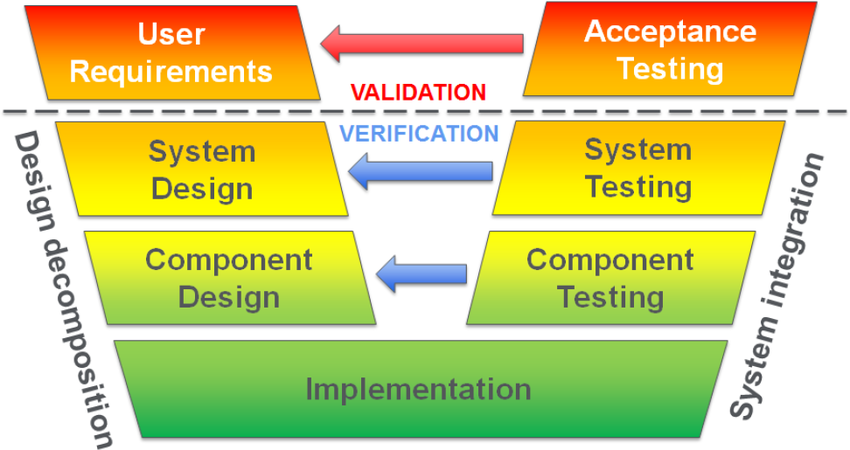
\includegraphics{v_model_methodology.png}
  \caption{Methodological framework based on the V-model from \glsentryshort{incose} with the different stages of the project development process\autocite{ruddle2020vmodel}}\label{fig:v_model_methodology}
\end{figure}

Moreover, a graphical representation of the V-model is provided in \cref{fig:v_model_methodology} to illustrate the methodology's structure and the relationship between the various stages.


\part{Theoretical Background}

\chapter{Non-Terrestrial Networks}\label{ch:non_terrestrial_networks}

As defined by the 3GPP \autocite{3gpp2018ntn}, an NTN refers to a network which partially/fully operates for communication purposes through a spaceborne vehicle (i.e., \gls{geo} and \gls{leo} satellites, or an airborne vehicle such as \glspl{hap} and \glspl{uav}). The most important feature that makes NTNs unique is their capability to provide connectivity in unreachable areas (for vessels, airplanes, etc.), or remote areas where a significant investment is required to build a terrestrial infrastructure.

\glspl{ntn} represent a groundbreaking approach in wireless communication, utilizing aerial and space-based platforms to deliver connectivity services. These platforms can operate at varying altitudes, from a range of a hundred meters to kilometers above ground, offering key advantages over traditional terrestrial networks, such as expanded coverage, increased capacity, and greater flexibility.

\glspl{ntn} provide a promising solution to meet the rising demand for wireless access in remote and underserved areas. By leveraging aerial and space platforms, \glspl{ntn} can extend the reach of conventional terrestrial networks, offering connectivity where traditional infrastructure is either difficult or impossible to deploy. In \cref{fig:ntn_types}, we illustrate the different types of \glspl{ntn} based on altitude and platform type as well as their interaction with other network elements such as \glspl{ue}, \gls{iot} devices, etc.

\section{Geostationary Satellites}

\gls{geo} satellites operate at an altitude of approximately \SI{36000}{\kilo\meter} above the Earth's equator. These satellites maintain a fixed position relative to the Earth’s surface, as they orbit at the same rate as the planet's rotation.\ \gls{geo} satellites offer extensive coverage, often spanning entire continents, and are widely used for telecommunications, broadcasting, and weather monitoring.

\gls{geo} satellites offer broad coverage and high capacity, making them ideal for applications like direct-to-home television, satellite radio, and broadband internet access. Their capacity to cover large regions makes \glspl{geo} integral to global communications infrastructure.

A key advantage of \gls{geo} satellites is their ability to support high-capacity services for many users, making them valuable for broadcasting live events, such as sports and concerts, or delivering high-definition video content worldwide. As a fundamental part of the global media and communication ecosystem, \gls{geo} satellites are expected to continue playing a vital role in providing connectivity to remote and underserved regions.

\section{Low-Earth Orbit Satellites}

\gls{leo} satellites operate at altitudes between \SI{160}{\kilo\meter} and \SI{2000}{\kilo\meter} above the Earth. Orbiting at high speeds, these satellites provide global coverage, making them ideal for delivering connectivity to remote and underserved regions.\ \gls{leo} satellites offer numerous advantages over traditional \gls{geo} satellites, including lower latency, higher capacity, and reduced infrastructure costs.

Deployed in constellations consisting of hundreds or thousands of satellites, \gls{leo} satellites work together to provide continuous coverage. These satellites communicate through inter-satellite links, allowing data to be relayed seamlessly across the constellation.\ \gls{leo} satellites are well-suited for delivering broadband internet access in areas where traditional infrastructure is difficult to establish.

One of the primary advantages of \gls{leo} satellites is their low latency, enabling real-time communication and supporting applications that require minimal delay, such as online gaming, video conferencing, and autonomous vehicle systems. Additionally, \gls{leo} satellites offer high-speed internet connectivity to users in remote locations, granting access to online services, educational platforms, and e-commerce opportunities. As a critical part of the emerging \gls{ntn} ecosystem, \gls{leo} satellites are expected to play a key role in bridging the global digital divide.

\section{High-Altitude Platforms}

\glspl{hap} operate at altitudes ranging from a hundred meters to kilometers above the Earth. These platforms may consist of balloons, airships, or \glspl{uav}. They provide unique benefits compared to traditional terrestrial networks, including broader coverage, increased capacity, and lower infrastructure costs.\ \glspl{hap} can be deployed swiftly to offer connectivity in remote or underserved areas, making them an effective tool for reducing the digital divide.

Additionally, \glspl{hap} can provide temporary connectivity in disaster-stricken regions or during large-scale events. Rapid deployment allows emergency responders to coordinate efforts efficiently. They can also extend the coverage of existing networks in rural areas, where conventional infrastructure is costly or challenging to install.

Advances in \gls{uav} technology have enabled the development of autonomous \glspl{hap} equipped with \gls{lte} or \gls{5g} base stations, flying at altitudes of up to \SI{20}{\kilo\meter}. These platforms cover substantial areas and support a range of applications, making them ideal for remote and underserved locations where deploying traditional infrastructure is not practical.

\begin{figure}
  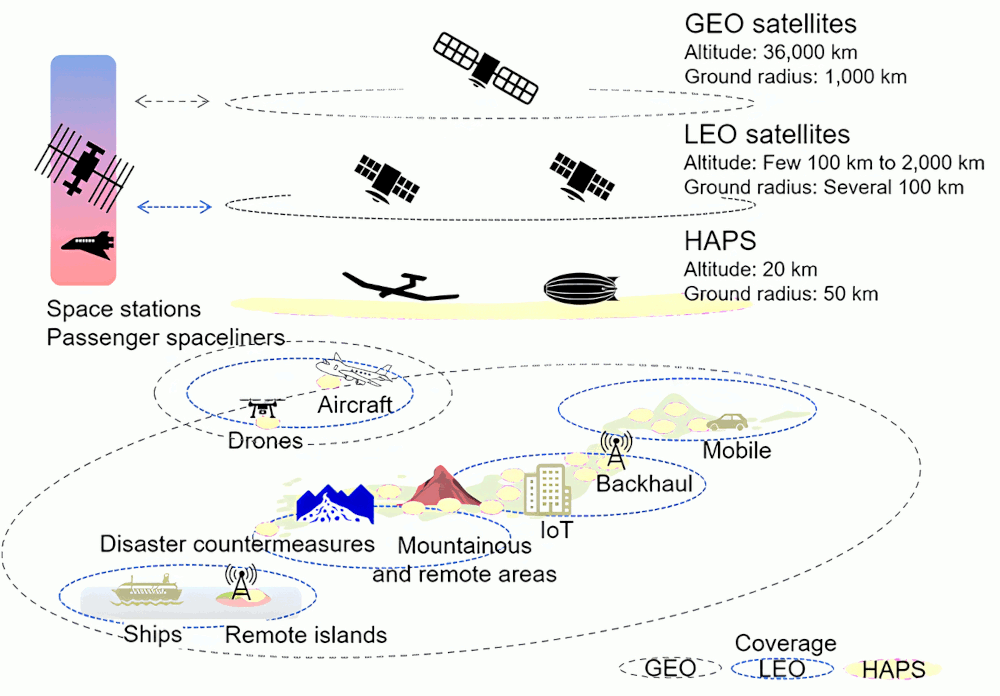
\includegraphics{non_terrestrial_networks_types.png}
  \caption{Types of \glsentryshortpl{ntn} based on altitude and platform type.\ \glsentryshortpl{hap}, \glsentryshortpl{leo} satellites, and \glsentryshortpl{geo} satellites interact with other network elements to provide connectivity services.\ \autocite{alertifyAirbusNTT}}\label{fig:ntn_types}
\end{figure}

% Local Variables:
% jinx-local-words: "alertifyAirbusNTT iot ntn spaceborne uav ue"
% End:

\chapter{Unmanned Aerial Vehicles}\label{ch:unmanned_aerial_vehicles}

The term \gls{uav} encompasses a diverse range of aircraft, from compact quad-copters to larger fixed-wing models. What primarily distinguishes \glspl{uav} from conventional aircraft is that \glspl{uav} are either remotely piloted or autonomously controlled, whereas traditional aircraft are operated by human pilots. This autonomy enables \glspl{uav} to be deployed in scenarios where human presence is either impractical or hazardous, such as military operations or environments with significant risk.

\glspl{uav} serve various purposes across multiple industries, including surveillance, reconnaissance, search and rescue missions, and scientific research. Additionally, they have become invaluable in sectors like agriculture, forestry, and environmental monitoring. In recent years, \glspl{uav} have gained popularity among hobbyists for recreational flying and personal projects.

\section{Types of Unnamed Aerial Vehicles}

In line with the classification presented by the \gls{easa} \autocite{eu-947-2019}, \glspl{uav} can be categorized into three main types, each based on size, weight, physical design, and operational capabilities:

\begin{itemize}
  \item \textbf{Fixed-wing \glspl{uav}:} These aircraft feature fixed wings and function similarly to conventional airplanes. They tend to be larger and designed for long-duration flights, making them suitable for extended missions like surveillance, reconnaissance, and mapping. However, they require runways for takeoff and landing, and cannot hover in place, limiting their versatility in confined spaces.

  \item \textbf{Rotary-wing \glspl{uav}:} Equipped with multiple rotors, these \glspl{uav} can take off and land vertically. They are typically smaller and more agile, making them ideal for close-range missions like aerial photography, search and rescue, and surveillance. However, their limited range and endurance compared to fixed-wing \glspl{uav} restrict their use in long-duration missions.

  \item \textbf{Hybrid \glspl{uav}:} Combining the features of both fixed-wing and rotary-wing designs, hybrid \glspl{uav} can take off and land vertically like rotary-wing models while achieving greater range and endurance through fixed-wing flight. These aircraft are ideal for missions requiring versatility, such as reconnaissance and mapping. Despite their advantages, they are more complex and costly to operate than single-type \glspl{uav}.
\end{itemize}

\Cref{fig:uav_types} illustrates the different \glspl{uav} types based on their design and intended applications.

\begin{figure}
  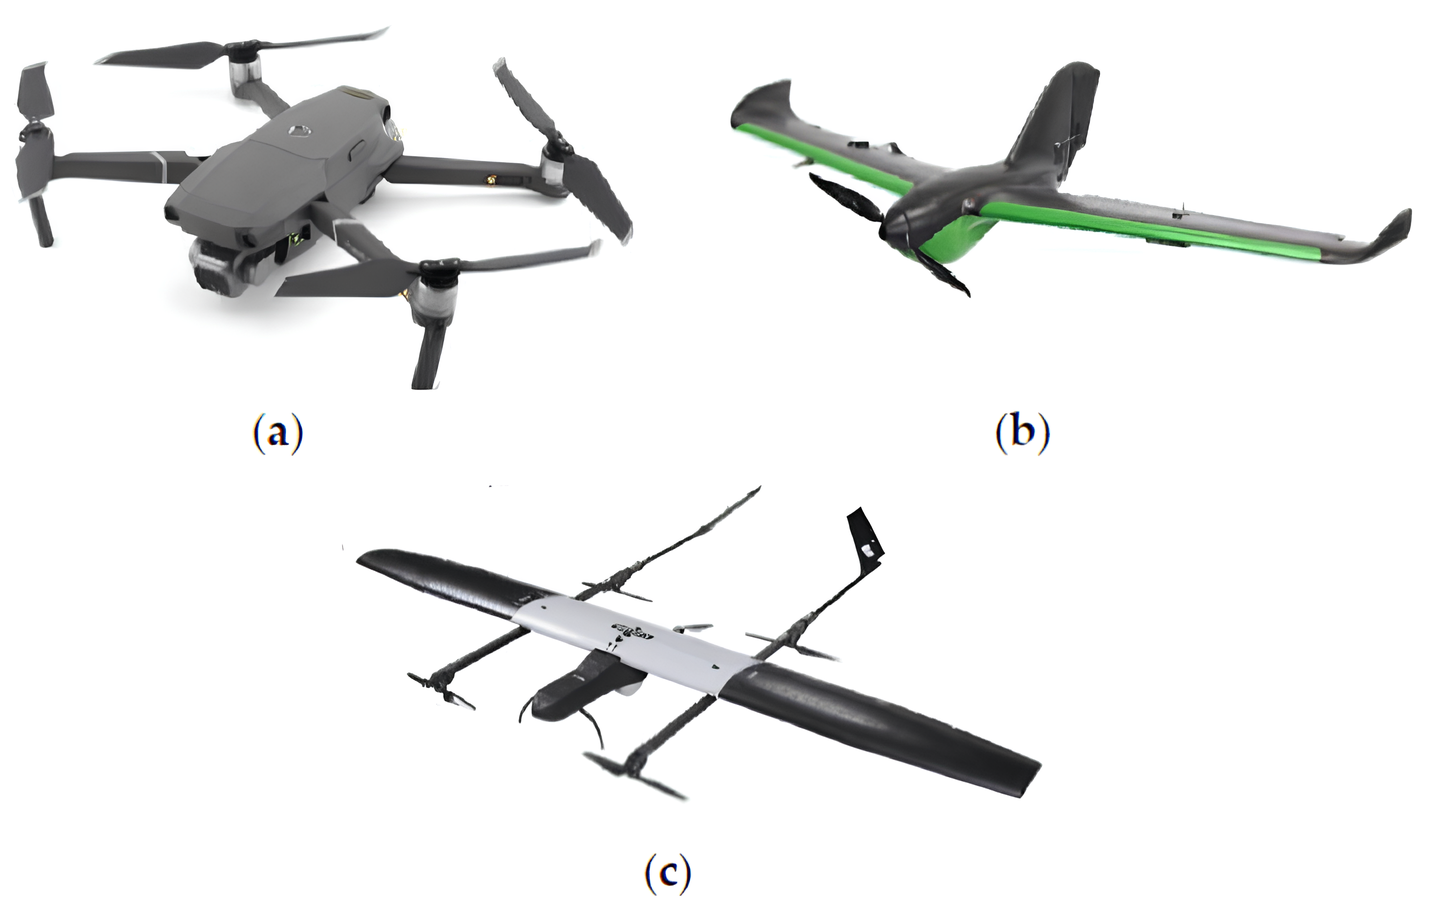
\includegraphics{uav_types.png}
  \caption{Types of \glsentryshortpl{uav} based on their design and intended use \autocite{mohnani2022role}.\ a. Rotary-wing \glsentryshort{uav}, b. Fixed-wing \glsentryshort{uav}, c. Hybrid \glsentryshort{uav}}\label{fig:uav_types}
\end{figure}

In \cref{tab:uav_categories}, a detailed comparison of fixed-wing, rotary-wing, and hybrid \glspl{uav} is presented across various performance metrics, including size, range, endurance, cost, and ease of operation. The table provides insights to help in selecting the appropriate \gls{uav} for specific mission requirements, depending on factors like payload, range, and maneuverability.

\begin{table}
  \begin{tabular}{ l c c c }
    \toprule
    \textbf{Metric} & \textbf{Fixed-wing} & \textbf{Rotary-wing} & \textbf{Hybrid} \\
    \midrule
    Size & Moderate & Small & Large \\
    Range & Long & Short & Moderate \\
    Endurance & High & Low & Moderate \\
    Payload capacity & High & Low & Moderate \\
    Maneuverability & Low & High & Moderate \\
    Ease of use & Moderate & High & Low \\
    Maintenance & Moderate & Low & High \\
    Runway requirement & Yes & No & Yes \\
    Cost & Moderate & Low & High \\
    \bottomrule
  \end{tabular}
  \caption{Comparison of fixed-wing, rotary-wing, and hybrid \glsentryshortpl{uav} across various performance metrics}\label{tab:uav_categories}
\end{table}

\section{Applications of Unmanned Aerial Vehicles}

\glspl{uav} have a wide range of applications across different industries, leveraging their versatility, maneuverability, and autonomy. Some common applications of \glspl{uav} include:

\begin{itemize}
  \item \textbf{Aerial photography and videography:} \glspl{uav} equipped with high-resolution cameras are used for capturing aerial images and videos for various purposes, including filmmaking, real estate, and landscape photography.

  \item \textbf{Agriculture:} \glspl{uav} are employed in precision agriculture to monitor crop health, assess soil conditions, and optimize irrigation and fertilization practices. They can provide valuable insights to farmers for improving crop yield and reducing resource wastage.

  \item \textbf{Search and rescue:} \glspl{uav} equipped with thermal imaging cameras and other sensors are used in search and rescue operations to locate missing persons, assess disaster-affected areas, and deliver essential supplies to remote locations.

  \item \textbf{Infrastructure inspection:} \glspl{uav} are utilized for inspecting critical infrastructure like bridges, power lines, and pipelines. They can access hard-to-reach areas and capture detailed images for assessing structural integrity and identifying maintenance needs.

  \item \textbf{Environmental monitoring:} \glspl{uav} are deployed for monitoring environmental parameters like air quality, water quality, and wildlife populations. They can collect data in remote or hazardous environments, providing valuable insights for conservation efforts and scientific research.

  \item \textbf{Disaster response:} \glspl{uav} play a crucial role in disaster response by providing real-time situational awareness, mapping affected areas, and coordinating emergency operations. They can assist in assessing damage, locating survivors, and delivering aid to disaster-stricken regions.

  \item \textbf{Military and defense:} \glspl{uav} are extensively used in military and defense applications for reconnaissance, surveillance, target acquisition, and combat operations. They offer a cost-effective and low-risk alternative to manned aircraft in high-risk environments.

    \item \textbf{Delivery services:} \glspl{uav} are increasingly being used for last-mile delivery of goods and services. Companies like Amazon and UPS are exploring the use of \glspl{uav} for delivering packages to customers in urban and rural areas.
\end{itemize}

% Local Variables:
% jinx-local-words: "easa uav"
% End:

\chapter{Deep Learning}\label{ch:deep_learning}

\gls{dl} is a subfield of \gls{ml} that focuses on the development of algorithms and models inspired by the structure and function of the human brain. These algorithms are designed to learn from data, identify patterns and relationships, and make predictions or decisions without explicit instructions.\ \gls{dl} algorithms are characterized by their ability to automatically discover and extract features from raw data, enabling them to perform complex tasks such as image recognition, speech recognition, and natural language processing.

\gls{dl} has revolutionized various industries and domains, including healthcare, finance, transportation, and entertainment. By leveraging the power of \gls{dl}, organizations can analyze large datasets, extract valuable insights, and automate complex tasks, leading to improved decision-making, enhanced user experiences, and optimized processes. From self-driving cars and virtual assistants to medical diagnostics and fraud detection, \gls{dl} is transforming the way we interact with technology and the world around us.

Furthermore, \gls{dl} plays a crucial role in enabling \gls{uav} autonomy, allowing drones to perform tasks such as navigation, obstacle avoidance, and object recognition without human intervention. By integrating \gls{dl} algorithms into \gls{uav} systems, researchers and developers can enhance the capabilities and efficiency of drones, enabling them to operate in complex environments and execute sophisticated missions.

\section{Deep Learning Techniques}

\gls{dl} encompasses a wide range of techniques and architectures that enable machines to learn from data and make decisions. Some of the most common \gls{dl} techniques include:

\begin{itemize}
  \item \textbf{\glspl{ann}:} \glspl{ann} are computational models inspired by the structure and function of the human brain. They consist of interconnected nodes, or neurons, organized in layers, with each neuron performing a simple computation.\ \gls{ann} can learn complex patterns and relationships in data through a process called back-propagation, where errors are propagated back through the network to adjust the model's parameters.\ \gls{ann} are used in a variety of tasks, such as classification, regression, and clustering.

  \item \textbf{\glspl{cnn}:} \glspl{cnn} are a type of \glspl{ann} designed for processing and analyzing visual data, such as images and videos. They use convolutional layers to extract features from input data, pooling layers to reduce spatial dimensions, and fully connected layers to make predictions.\ \gls{cnn} are widely used in image recognition, object detection, and image segmentation tasks.

  \item \textbf{\glspl{rnn}:} \glspl{rnn} are a type of \glspl{ann} designed for processing sequential data, such as time series, text, and speech. They have feedback connections that allow information to persist over time, enabling them to capture temporal dependencies in data.\ \gls{rnn} are used in natural language processing, speech recognition, and machine translation tasks.

  \item \textbf{\glspl{gan}:} \glspl{gan} are a type of a \gls{dl} model that consists of two neural networks, a generator and a discriminator, trained adversarially. The generator generates synthetic data samples, while the discriminator distinguishes between real and fake samples.\ \gls{gan} are used in image generation, style transfer, and data augmentation tasks.
\end{itemize}

These techniques form the foundation of \gls{dl} and are used in a wide range of applications across various domains, enabling machines to perform complex tasks and make intelligent decisions. In the context of \gls{ntn} and \glspl{uav}, \gls{dl} techniques can enhance network performance, optimize resource allocation, and enable autonomous operation, leading to more efficient and reliable systems. Furthermore, \gls{dl} can enable \glspl{uav} to perform tasks such as navigation, object detection, and mission planning with high accuracy and efficiency, making them valuable tools for a wide range of applications (e.g., surveillance, monitoring, and disaster response).


\part{State of the art}

\chapter{Historical Development}\label{ch:historical_development}

The evolution of \glspl{ntn} and \glspl{uav} has been shaped by technological advances and the increasing demand for global connectivity over the past several decades. Originally, \glspl{ntn}, encompassing satellite communication networks, \glspl{hap}, and \glspl{uav}, were developed for specialized applications. These early systems were primarily used for military, navigation, television broadcasting, remote sensing, and disaster management purposes. Due to the high costs and complexities associated with the manufacturing, launching, and maintaining these systems, their deployment was limited to specific sectors and regions, often focusing on government or large corporate projects.

Early satellite communication networks were dominated by \gls{geo} satellites, which provided consistent coverage over specific areas of the Earth, particularly for television broadcasting and weather forecasting. However, the high latency and large round-trip time associated with \gls{geo} satellites, positioned at approximately \SI{36000}{\kilo\meter} from Earth, posed challenges for expanding their use to real-time communication services. Additionally, the prohibitive costs and challenges of deploying and maintaining \gls{geo} satellites restricted their usage largely to commercial and government-backed projects.

Throughout the late 20th century, \glspl{ntn} remained niche solutions, but technological advancements and the growing need for more comprehensive and reliable global connectivity shifted the focus. The limitations of \glspl{tn}, particularly in rural, remote, and inaccessible regions such as deserts, oceans, and mountainous areas, drove the demand for new approaches. Expanding terrestrial network coverage into these regions posed economic and logistical challenges, making \glspl{ntn} a critical complementary solution. Satellites became vital to extending coverage beyond the reach of terrestrial infrastructure, filling gaps where ground-based systems were either impractical or uneconomical to deploy.

The 1990s saw the rise of \gls{leo} satellite constellations, which were developed to overcome some of the inherent limitations of \gls{geo} satellites.\ \gls{leo} satellites, operating at much lower altitudes of \SI{300}{\kilo\meter} to \SI{1500}{\kilo\meter}, offered significantly reduced latency and improved spectral efficiency. These benefits made \gls{leo} satellites more suitable for supporting new and emerging applications that demanded real-time communication and data transmission. Despite the technological promise of \gls{leo} satellites, the initial wave of mega-constellation projects—large networks comprising hundreds to thousands of satellites—stalled, largely due to the high costs of deployment and a lack of sustainable business models.

The late 1990s and early 2000s marked a renewed interest in integrating \glspl{ntn} with terrestrial systems, particularly as global internet access became a key societal goal. As mobile network generations progressed from \gls{2g} to \gls{4g}, the need for more adaptive network solutions grew. However, it was not until the development of \gls{5g}, spearheaded by the \gls{3gpp}, that serious efforts were made to fully integrate \glspl{ntn} with terrestrial networks.\ \gls{3gpp}'s Release 15 \autocite{3gpp_rel15} in 2018 laid the foundation for \gls{5g} networks, and subsequent releases aimed to include \glspl{ntn}, such as satellite and \glspl{hap}, as essential components of the \gls{5g} ecosystem. These efforts recognized \glspl{ntn}' potential to expand the reach of \gls{5g} networks into underserved areas and enhance service reliability in mobile broadband and \gls{iot} applications.

During the same period, advancements in \glspl{uav} also contributed to the development of \glspl{ntn}. Initially developed for military and surveillance applications, \glspl{uav} began to be explored for their potential in civil applications such as disaster management, agriculture, and communications. The rise of \gls{5g} networks allowed for \glspl{uav} to be integrated into terrestrial networks, enabling beyond \gls{vlos} operations that required low-latency, reliable connections for autonomous vehicles, precision agriculture, and more.

As \gls{5g} networks continue to evolve, \glspl{ntn} are becoming increasingly vital in ensuring seamless global connectivity.\ \gls{leo} constellations, in particular, have seen a resurgence, with companies like SpaceX (Starlink) \autocite{tao2022impact} and OneWeb \autocite{zhu2022laser} developing large satellite networks to deliver low-latency, high-speed internet services to remote areas. These \glspl{ntn} are providing the much-needed infrastructure to bridge the digital divide by offering global coverage, enhancing reliability, and addressing specific issues such as network scalability and latency that have traditionally limited satellite communications.

% Local Variables:
% jinx-local-words: "iot ntn uav"
% End:

\chapter{Types \& Technologies}
\label{ch:types_technologies}

\todo{write this chapter}

\chapter{Modern Trends}\label{ch:modern_trends}

\todo{write this chapter}

% https://www.mdpi.com/2504-446X/6/11/334/xml
% 2. structure of ntns and key technologies, really good

% https://www.sciencedirect.com/science/article/pii/S1389128620311324?casa_token=Gd8qu0RsSOMAAAAA:g5pqykl8Q0xex2YlrWap6q81Os1YAo0V7708bDCw-H_gmeVZFX-GABzvb4rvxheuXal0YFArAw
% drone networks

% https://ieeexplore.ieee.org/stamp/stamp.jsp?tp=&arnumber=9768113

% https://ieeexplore.ieee.org/stamp/stamp.jsp?tp=&arnumber=9889300
% uav use cases in ntn

% https://ieeexplore.ieee.org/stamp/stamp.jsp?tp=&arnumber=9681624
% uavs and beyond

% https://ieeexplore.ieee.org/stamp/stamp.jsp?tp=&arnumber=10500741
% how uavs can be used in ntn

\chapter{Regulatory Framework}
\label{ch:regulatory_framework}

The regulatory framework governing drones is a complex and dynamic area, influenced by various laws and regulations that differ from country to country. Generally, drone operations are regulated by aviation authorities responsible for ensuring safe and responsible usage.

\section{Relevant Institutions}

\subsection{European Union Aviation Safety Agency (EASA)}
The European Union Aviation Safety Agency (EASA) \autocite{eu-1139-2018} plays a crucial role in harmonizing aviation safety standards across all EU member states. Its primary objective is to maintain a consistent and high level of safety in civil aviation operations throughout the European Union. EASA achieves this through the establishment and enforcement of common regulations applicable to all member states. Notably, for the standardization of Unmanned Aerial Systems (UAS), EASA has implemented Regulations (EU) 2019/947 \autocite{eu-947-2019} and (EU) 2019/945 \autocite{eu-945-2019}.

\subsection{Spanish Aviation Safety and Security Agency (AESA)}
In Spain, the Spanish Aviation Safety and Security Agency (AESA) \autocite{sp-184-2008} serves as the national regulatory authority, overseeing compliance with civil aviation standards within the aerospace sector. AESA plays a critical role in promoting the development and application of aviation legislation, ensuring that the Spanish civil aviation system upholds the highest safety, quality, and sustainability standards. In instances of non-compliance with aviation regulations, AESA possesses the authority to enforce sanctions.

\section{Applicable Legislation}

\subsection{Implementing Regulation (EU) 2019/947}
The Implementing Regulation (EU) 2019/947 \autocite{eu-947-2019} establishes the operational rules and requirements for UAS within the European Union. It provides a legal framework for the utilization of UAS across various operational categories, outlining requirements for operational authorizations and risk assessments where applicable. The regulation sets standards for remote pilot competency, operational procedures, and safety management to conduct UAS flights safely and effectively.

Additionally, it integrates with the Delegated Regulation (EU) 2019/945 \autocite{eu-945-2019} by defining operational requirements related to the UAS classes established within it. The regulation details specific operational limitations and conditions for each UAS class, including the management of UAS in classes C0 through C4. It also includes provisions for the safe integration of newly introduced UAS classes under Delegated Regulation (EU) 2020/1058 \autocite{eu-1058-2020}, specifically classes C5 and C6.

Moreover, this regulation addresses the procedures for UAS operators from third countries (non-EASA member states) wishing to operate within the Single European Sky (SES) airspace, ensuring alignment with EU standards and safety regulations.

\subsection{Delegated Regulation (EU) 2019/945}
The Delegated Regulation (EU) 2019/945 \autocite{eu-945-2019} defines the rules and standards for UAS within the European Union. It specifies the types of UAS that require certification regarding design, production, and maintenance. This regulation also provides guidelines for the commercialization of UAS intended for use in the Open category, as well as for remote identification accessories (e.g., Drone Remote ID). Furthermore, it outlines the requirements for the design and manufacture of UAS intended for operations defined in the Implementing Regulation (EU) 2019/947.

\subsection{Regulation (EU) 2024/1689: Artificial Intelligence Act}
The Artificial Intelligence Act (AI Act) of the European Union \autocite{AIActIntoForce}, which came into force on the 1st of August 2024, aims to ensure that AI systems are safe, transparent, and ethical, while fostering innovation and protecting fundamental rights as stated in the Delegated Regulation (EU) 2024/1689 \autocite{eu-1689-2024}. The Act categorizes AI systems by risk, imposing strict requirements on high-risk applications, particularly in aviation, which may affect public safety and fundamental rights. These requirements encompass robust risk management, transparency, human oversight, and data governance, ensuring that AI systems are reliable and secure.

The AI Act introduces significant compliance obligations that could escalate development costs and timelines. High-risk systems must adhere to stringent standards to access the EU market, potentially challenging innovation but ultimately aiming to build trust and facilitate broader adoption of AI technologies within the EU.

\section{Operational Categories}
The Regulation (EU) 2019/947 \autocite{eu-947-2019} classifies UAS into three distinct categories:

\begin{itemize}
  \item \textbf{Open Category:} The least restrictive category, designed for low-risk operations, includes activities such as recreational flying and commercial operations posing minimal risk to people and property. Operators must adhere to specific limitations (e.g., flying below 120 meters, maintaining Visual Line of Sight). UAS must weigh under 25 kg, and pilots must ensure that the drone does not fly over people or in restricted areas. No prior authorization is required, though registration and remote pilot training are compulsory for all operations, except for drones weighing less than 250 g that lack a camera or sensor.

  \item \textbf{Specific Category:} This category covers medium-risk operations necessitating a more detailed assessment. It includes operations that may involve flying over people or in restricted areas, provided mitigation procedures are in place. Operators must conduct a risk assessment and obtain an operational authorization known as Standard Training Scenarios (STS) from AESA. Requirements for UAS and pilot qualifications may vary based on the specific risk assessment and operational procedures defined within it.

  \item \textbf{Certified Category:} Designed for high-risk operations, this category involves stringent requirements comparable to those for manned aviation. UAS must meet specific certification standards and operators must comply with strict safety regulations. This category often includes advanced training requirements and operational procedures similar to those for commercial air transport.
\end{itemize}

\subsection{Open Category}
This work will focus on civil UAS that fall under EASA's Open Category, although some findings may be applicable to other categories with appropriate regulatory adjustments. Within the Open Category, three subcategories differentiate based on associated risk, aircraft weight, and operational limits:

\begin{enumerate}
  \item \textbf{A1}: UAS with a Maximum Takeoff Weight (MTOW) of less than 250 g that can fly over people but not over assemblies of people.

  \item \textbf{A2}: UAS with an MTOW of less than 4 kg that can fly close to people but must maintain a horizontal distance of 30 meters (5 meters in low-speed configuration).

  \item \textbf{A3}: UAS with an MTOW of less than 25 kg that must maintain a horizontal distance of 150 meters from residential, commercial, industrial, or recreational areas.
\end{enumerate}

Check \cref{fig:eu_regulations_open_category_chart} for a visual representation of the Open Category subcategories.

\begin{figure}
  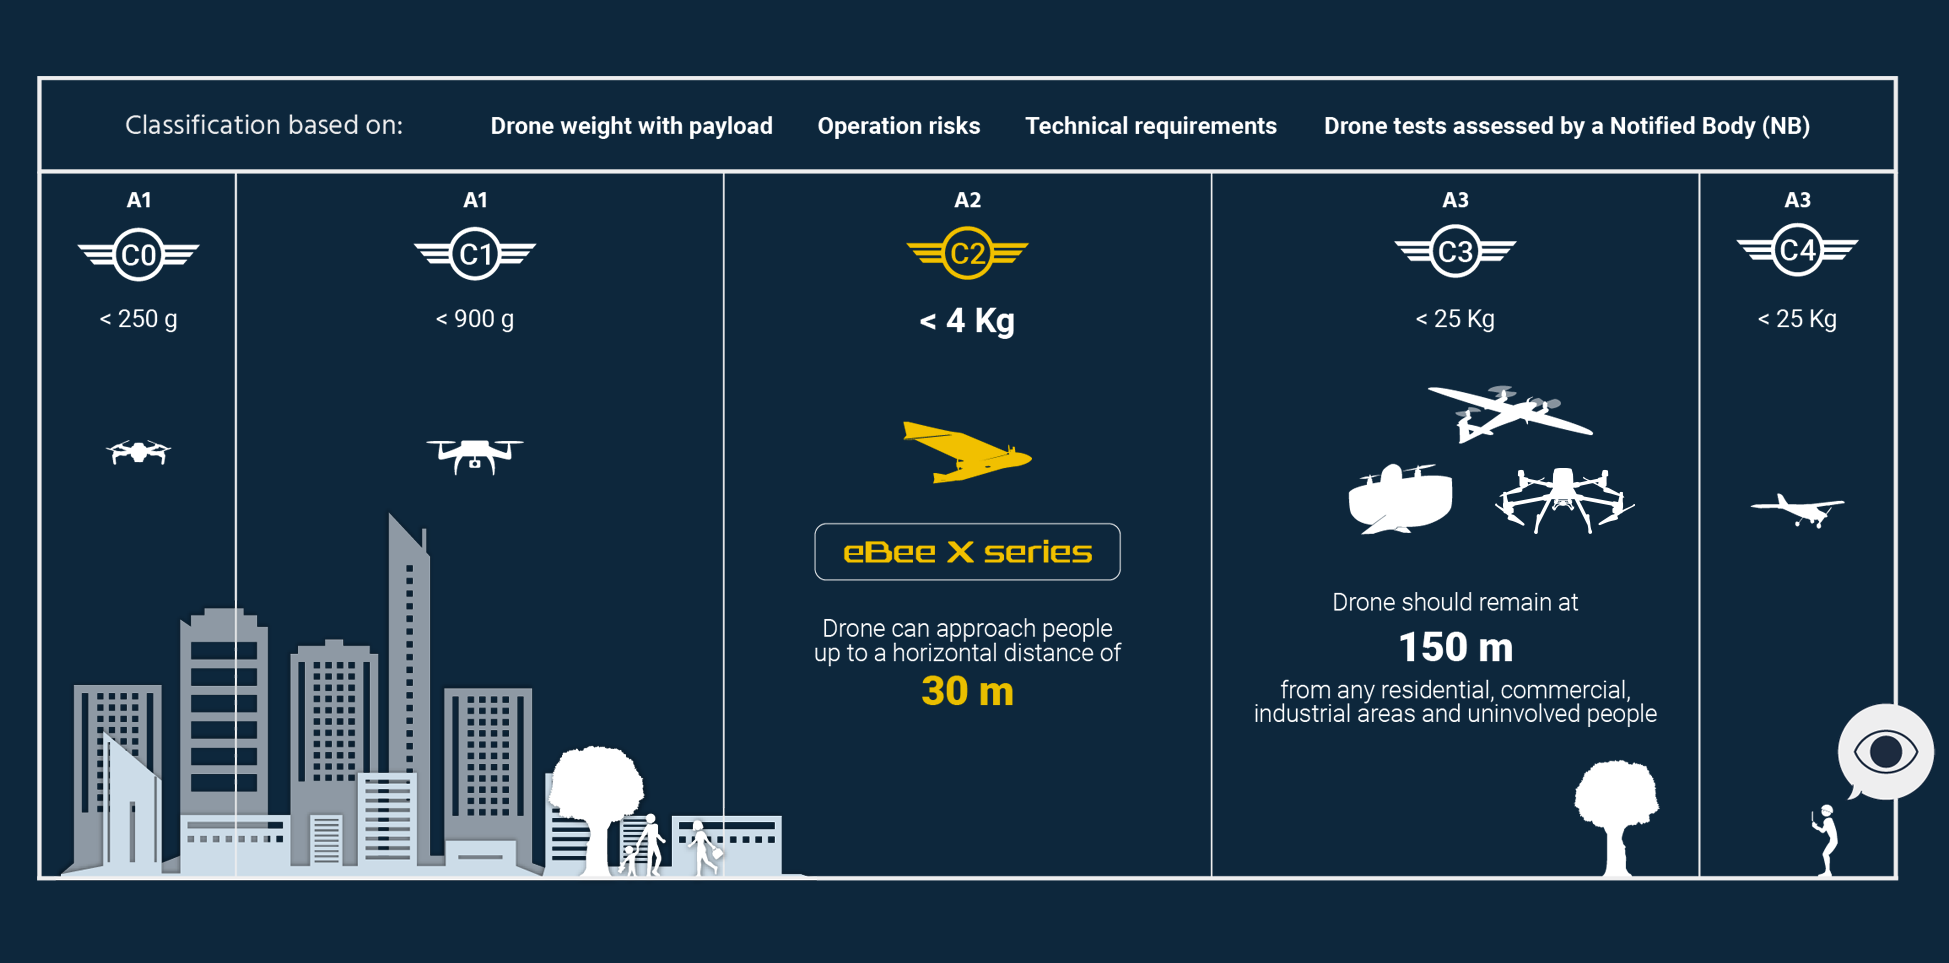
\includegraphics{eu_regulations_open_category_chart.png}
  \caption{EU Regulations Open Category chart describing the subcategories A1, A2, and A3 with their respective operational limitations \autocite{ageagleEuropeanUnion}}
  \label{fig:eu_regulations_open_category_chart}
\end{figure}

Moreover, additional rules applicable to all three subcategories include:

\begin{itemize}
  \item The maximum height must not exceed 120 meters above ground level, as the lower limit for general aviation is 150 meters. This leaves only a 30-meter separation between manned aviation and UAS.

  \item Operators must always maintain Visual Line of Sight (VLOS) unless the aircraft is in ``follow me'' mode or the pilot is using First-Person View (FPV) goggles.

  \item Operators must register if the UAS weighs more than 250 g or if the aircraft is equipped with a camera or sensor.

  \item The aircraft must possess a remote identification ID, which is standard in all C1-C6 categories, with the exception of C4 and privately built aircraft.
\end{itemize}


\part{Methodology}

\chapter{Requirements}

Based on careful analysis of the conclusions from the current trends in \glspl{uav} outlined in \cref{ch:modern_trends} and the objectives reviewed in \cref{ch:objectives}, the following requirements are established for the high-level system as well as the detailed requirements for the \gls{uav}, control station, and software platform.

\section{High-level System Requirements}

The high-level system requirements are as follows:

\begin{itemize}
  \item The system must be able to operate in remote areas with limited infrastructure, such as roads, electricity, and internet connectivity.

  \item The system must be able to be monitored remotely, with the ability to communicate with a ground station via a \gls{4g} or \gls{3g} connection.

  \item The system must be cost-effective, with the ability to be assembled and disassembled easily, and to be repaired and maintained with minimal effort.

  \item The system must be modular, allowing for the integration of different sensors and payloads for different applications, as well as, the scalability of the system to include multiple \glspl{uav} working together in a coordinated manner.

  \item The system must be able to perform reconnaissance tasks autonomously, with the ability to take off, land, and navigate given a set of waypoints.

  \item The system must comply with the applicable regulatory framework for \glspl{uav} in the country of operation, Spain, as well as the \gls{eu} regulations. See \cref{ch:regulatory_framework} for more information.
\end{itemize}

\section{Unmanned Aerial Vehicle Requirements}

The \gls{uav} requirements are as follows:

\begin{itemize}
  \item The \gls{uav} must be able to be controlled remotely, with the ability to communicate with a ground station in real-time.

  \item The \gls{uav} must be able to take off, land, and navigate autonomously, with the ability to update its flight plan in real-time.

  \item The \gls{uav} must be able to process data in real-time, with the ability to relay the information to the ground station.

  \item The \gls{uav} must be able to carry different payloads and sensors for different applications up to a maximum payload weight of 2 kg, with the ability to adapt to different reconnaissance tasks.

  \item The \gls{uav} must be able to fly for a minimum of 30 minutes, without the need for recharging.

  \item The \gls{uav} must be have a failsafe mechanism, that is it must be able to return to the ground station in case of loss of communication or other critical failures.

  \item The \gls{uav} must be able to keep a fixed altitude and position.

  \item The \gls{uav} must comply with the EASA regulations for the Open Category, with a maximum limit set at 25 kg of MTOW and 3 meters of wingspan.

  \item The \gls{uav} must be able to perform reconnaissance tasks, such as mapping, surveillance, and monitoring the environment.
\end{itemize}

\section{Control Station Requirements}

The control station requirements are as follows:


\begin{itemize}
  \item The control station must be able to receive telemetry data from the \gls{uav} in real-time, with the ability to send commands to the \gls{uav} to update its flight plan.

  \item The control station must be able to be used remotely, with the ability to communicate with the \gls{uav} via a \gls{4g} or \gls{3g} connection.

  \item The control station must be able to create a geofence around the area of operation, with the ability to monitor the \gls{uav}'s position and altitude in real-time.

  \item The control station must have the capability be able to track multiple \glspl{uav} simultaneously, with the ability to coordinate their flight plans and tasks.

  \item The control station must log all telemetry data and flight information, with the ability to analyze the data and generate reports.
\end{itemize}

\section{Software Platform Requirements}

The software platform requirements are as follows:

\begin{itemize}
  \item The software platform must be able to run on a variety of operating systems, with the ability to communicate with the \glspl{uav} and the control station in real-time.

  \item The software platform must be able to be used remotely, with the ability to access the \glspl{uav} and the control station via a \gls{4g} or \gls{3g} connection.

  \item The software platform must be reliable, secure, and easy to use, allowing for the programming of the \glspl{uav} to perform specific tasks and the coordination of multiple \glspl{uav} in a swarm.

  \item The software platform must be customizable, allowing for the integration of new features and the modification of existing ones, as well as, the addition of new \glspl{uav} to the system and different types of reconnaissance tasks.

  \item The software platform must have alerting and notification capabilities, with the ability to send alerts and notifications to the user in case of critical events or failures.

  \item The software platform must have a user-friendly interface, with the ability to display telemetry data and flight information in real-time, as well as, the ability to monitor the \glspl{uav} in real-time.
\end{itemize}

\chapter{Design}
\label{ch:design}

\todo{write this chapter}

\chapter{Implementation}\label{ch:implementation}

Following the design presented in the previous chapter, this chapter lays out the implementation of the system and the integration of the components that compose it, as well as the methodologies and tools used to develop, assemble, and integrate the system. As stated in the design chapter, refer to \cref{ch:design}, the system is divided into four main components: the \gls{uav}, the control station, the reconnaissance platform, and the communication system. Each component is implemented separately and then integrated into the system as a whole.

\section{Unmanned Aerial Vehicle}\label{sec:implementation_uav}

The \gls{uav} is the base platform and the main component of the system. For this reason, it is the first component to be implemented. The \gls{uav} is responsible for carrying the reconnaissance platform and the communication system, as well as for executing the flight plan generated by the control station. The detailed implementation of the \gls{uav} is out of the scope of this thesis and only a high-level overview of the implementation is provided. However, more information about the implementation of the \gls{uav} can be found in the \autocite{developingcosteffectivedrones5g}. Each subsystem of the \gls{uav} described in the \cref{sec:design_uav}
is implemented separately and then integrated into the \gls{uav} as a whole.

\subsection{Airframe}\label{subsec:implementation_airframe}

For the airframe, the \gls{uav} was built using following the instructions provided by the manufacturer. The airframe can be seen in \cref{fig:airframe}. However, some modifications were made to the airframe to accommodate the additional components using custom 3D printed parts (e.g., the landing gear, the camera mount, and the payload bay). The design and manufacture of the 3D printed parts where made using the FreeCAD software \autocite{freecadFreeCADYour} and a Bamboo P1S 3D printer \autocite{bambulabBambuPrinter}. The reason to use 3D printed parts is that they are easy to design and manufacture, as well as being lightweight and durable. The 3D printed parts were designed to be easily attached to the airframe using screws and nuts, as well as to be easily removed in case of maintenance or replacement. Some of the 3D printed parts used in the airframe can be seen in \cref{fig:3d_printed_landing_gear_stl}.

\begin{figure}
  \begin{subfigure}{0.4\textwidth}
    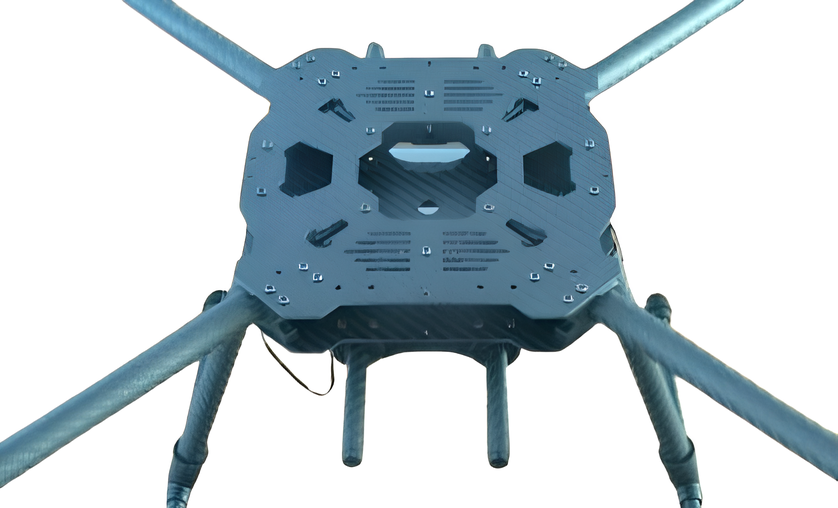
\includegraphics{airframe_tarot.png}
    \caption{Tarot XS690 airframe \autocite{developingcosteffectivedrones5g}.}\label{fig:airframe}
  \end{subfigure}
  \hfill
  \begin{subfigure}{0.4\textwidth}
    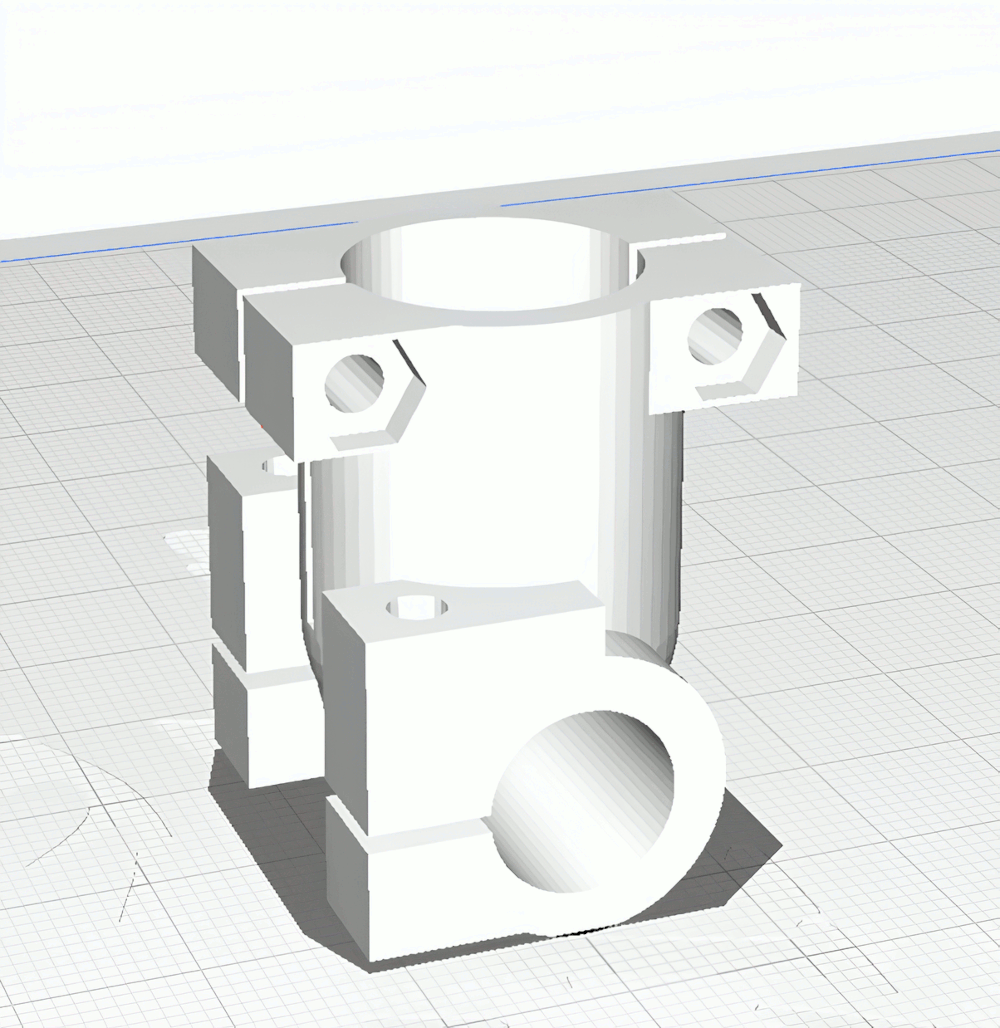
\includegraphics{3d_printed_landing_gear_stl.png}
    \caption{3D printed landing gear \autocite{developingcosteffectivedrones5g}.}\label{fig:3d_printed_landing_gear_stl}
  \end{subfigure}

  \caption{Airframe and 3D printed parts.}\label{fig:airframe_and_3d_printed_parts}
\end{figure}

\subsection{Propulsion System}\label{subsec:implementation_propulsion_system}

Regarding the propulsion system, the four motors were attached to the airframe using custom metal brackets, as seen in \cref{fig:motors_attached_to_airframe}. The \glspl{esc} were attached to the airframe using double-sided tape and zip ties, as seen in \cref{fig:esc_attached_to_airframe}.

\begin{figure}
  \hfill
  \begin{subfigure}{0.4\textwidth}
    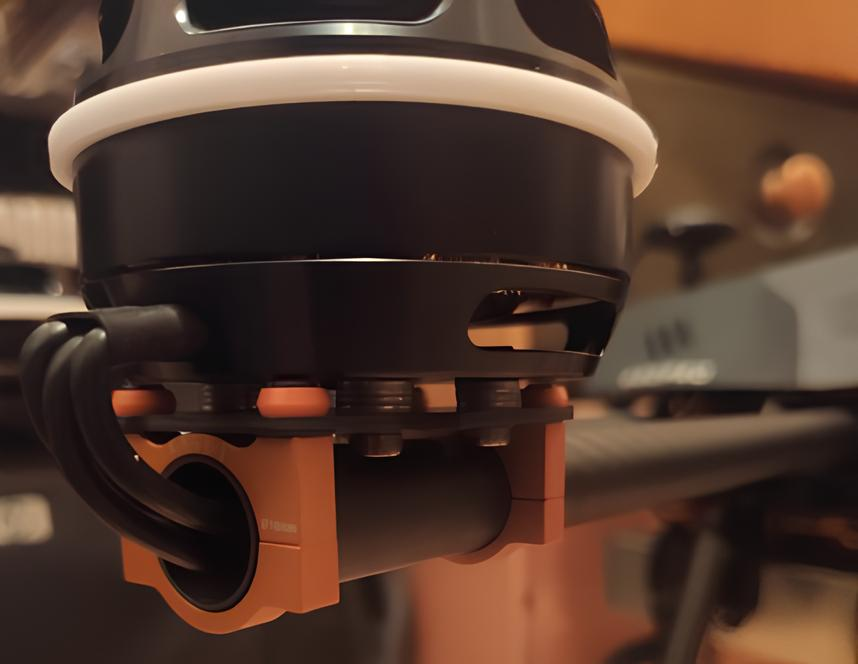
\includegraphics{motor_mount.jpg}
    \caption{Metal motor mount brackets to attach the motors to the airframe (orange brackets) \autocite{developingcosteffectivedrones5g}.}\label{fig:motors_attached_to_airframe}
  \end{subfigure}
  \hfill
  \begin{subfigure}{0.4\textwidth}
    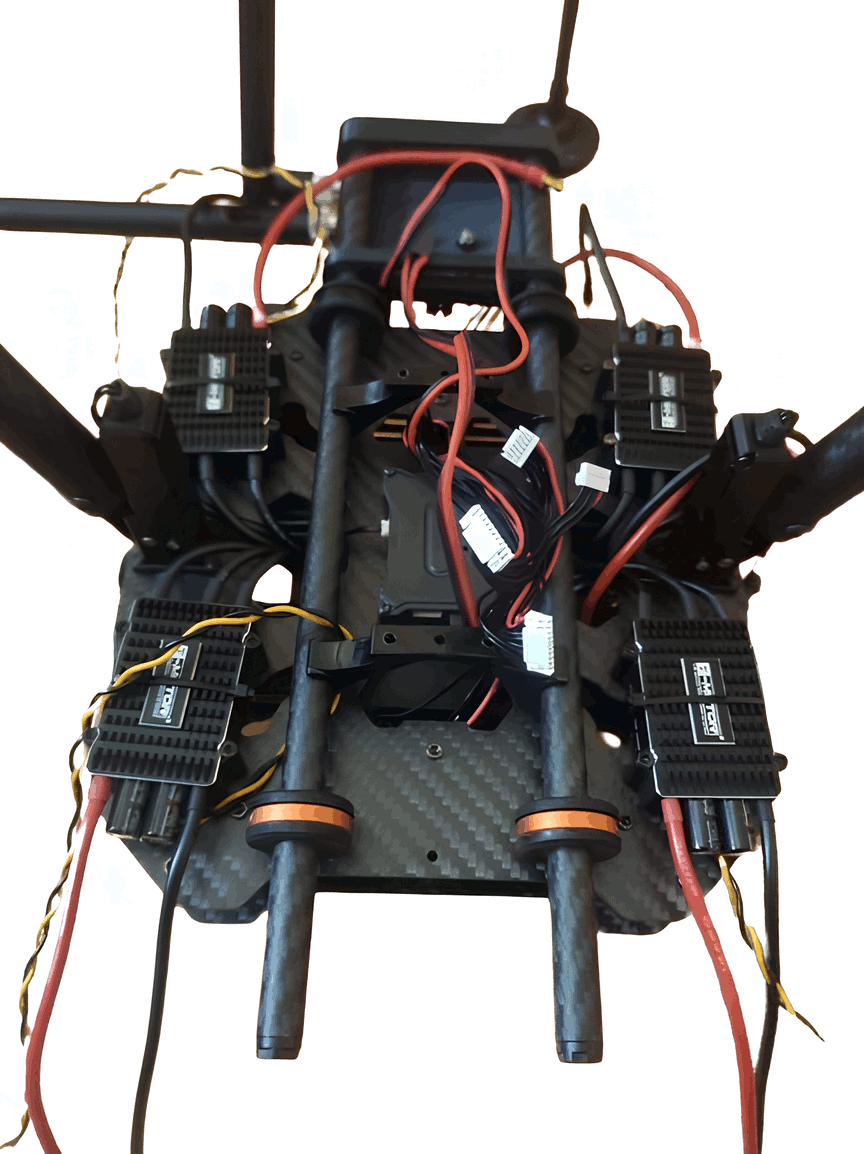
\includegraphics{bottom_plate_esc.png}
    \caption{Bottom view of the airframe with the \glspl{esc} attached in each corner \autocite{developingcosteffectivedrones5g}.}\label{fig:esc_attached_to_airframe}
  \end{subfigure}
  \hfill

  \caption{Propulsion system components attached to the airframe.}\label{fig:propulsion_system_components_attached_to_airframe}
\end{figure}

\subsection{Flight Controller}\label{subsec:implementation_flight_controller}

For the flight controller, it was placed in the middle of the airframe using double-sided tape and zip ties, as seen in \cref{fig:flight_controller_attached_to_airframe}. It is important to note that placing the flight controller in the middle of the airframe provides the best balance and stability for the \gls{uav} during flight.

\begin{figure}
  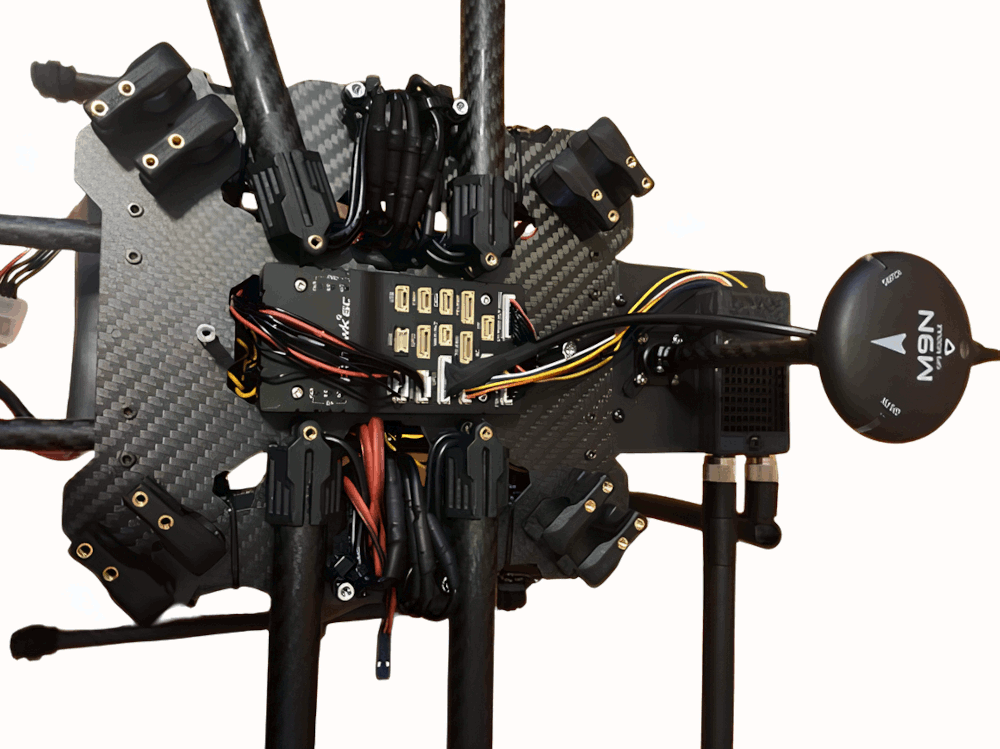
\includegraphics[width=0.4\textwidth]{mid_plate_flight_controller.png}
  \caption{Flight controller attached to the airframe in the middle of the airframe \autocite{developingcosteffectivedrones5g}.}\label{fig:flight_controller_attached_to_airframe}
\end{figure}

\subsection{Power System}\label{subsec:implementation_power_system}

The power system is the heaviest subsystem of the \gls{uav} and must be placed in the center of the airframe to provide the best balance and stability during flight. The battery was attached to the airframe using battery straps, as seen in \cref{fig:battery_attached_to_airframe}. The \gls{pdb}, \cref{fig:pdb}, was attached to the airframe using a custom 3D printed mount and places in the middle of the airframe, as seen in \cref{fig:power_distribution_board_attached_to_airframe}. Also, the voltage regulator was attached to the top of the airframe using double-sided tape and zip ties, refer to \cref{fig:computer_attached_to_airframe}.

\begin{figure}
  \hfill
  \begin{subfigure}[t]{0.3\linewidth}
    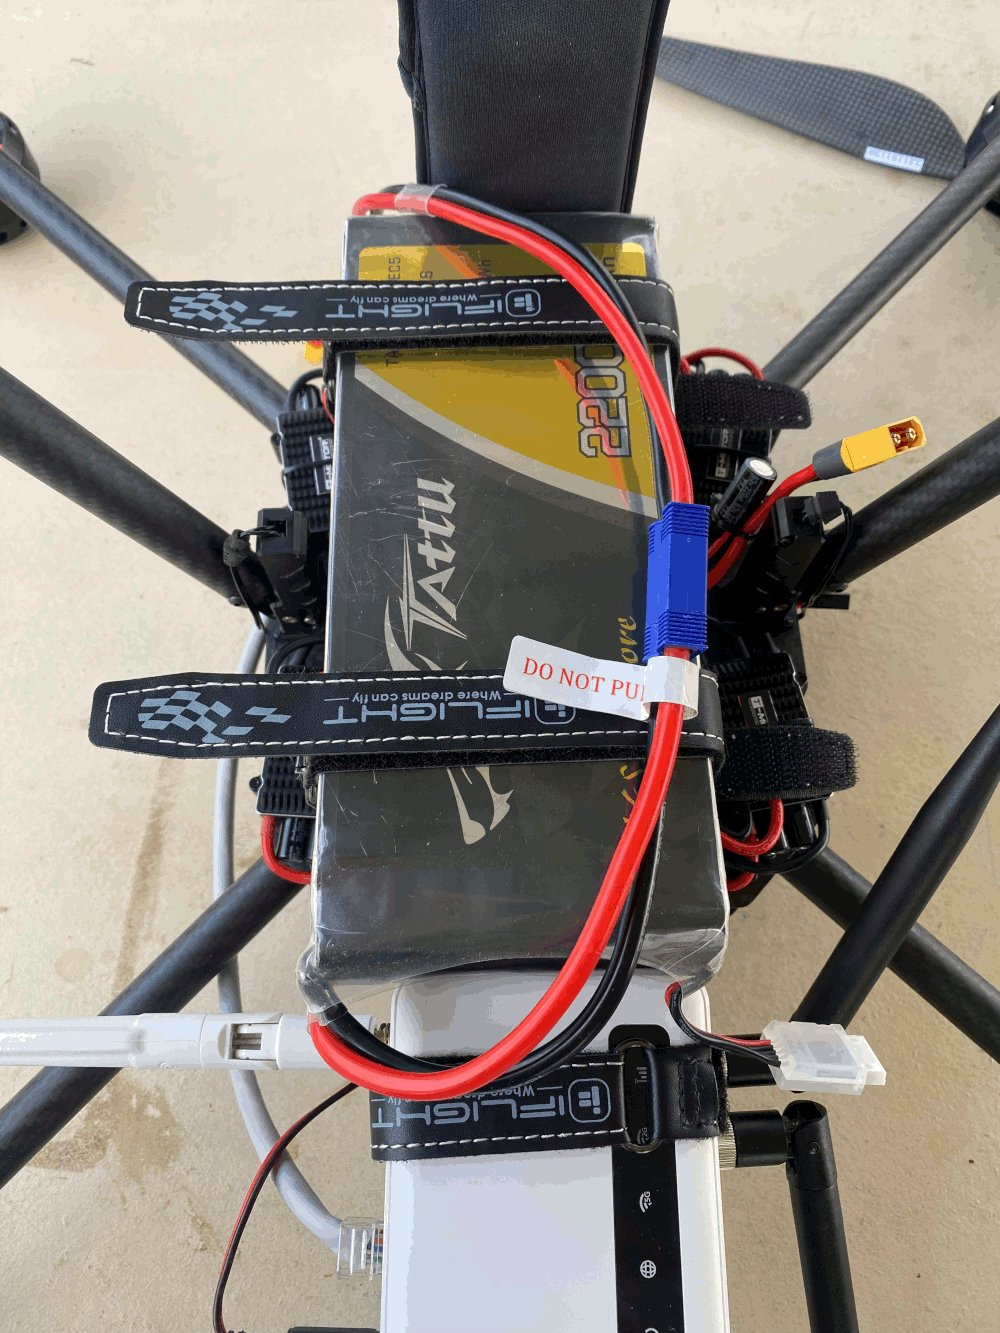
\includegraphics[width=\linewidth]{bottom_plate_battery.jpg}
    \caption{Battery attached to the airframe.}\label{fig:battery_attached_to_airframe}
  \end{subfigure}
  \hfill
  \begin{subfigure}[t]{0.3\linewidth}
    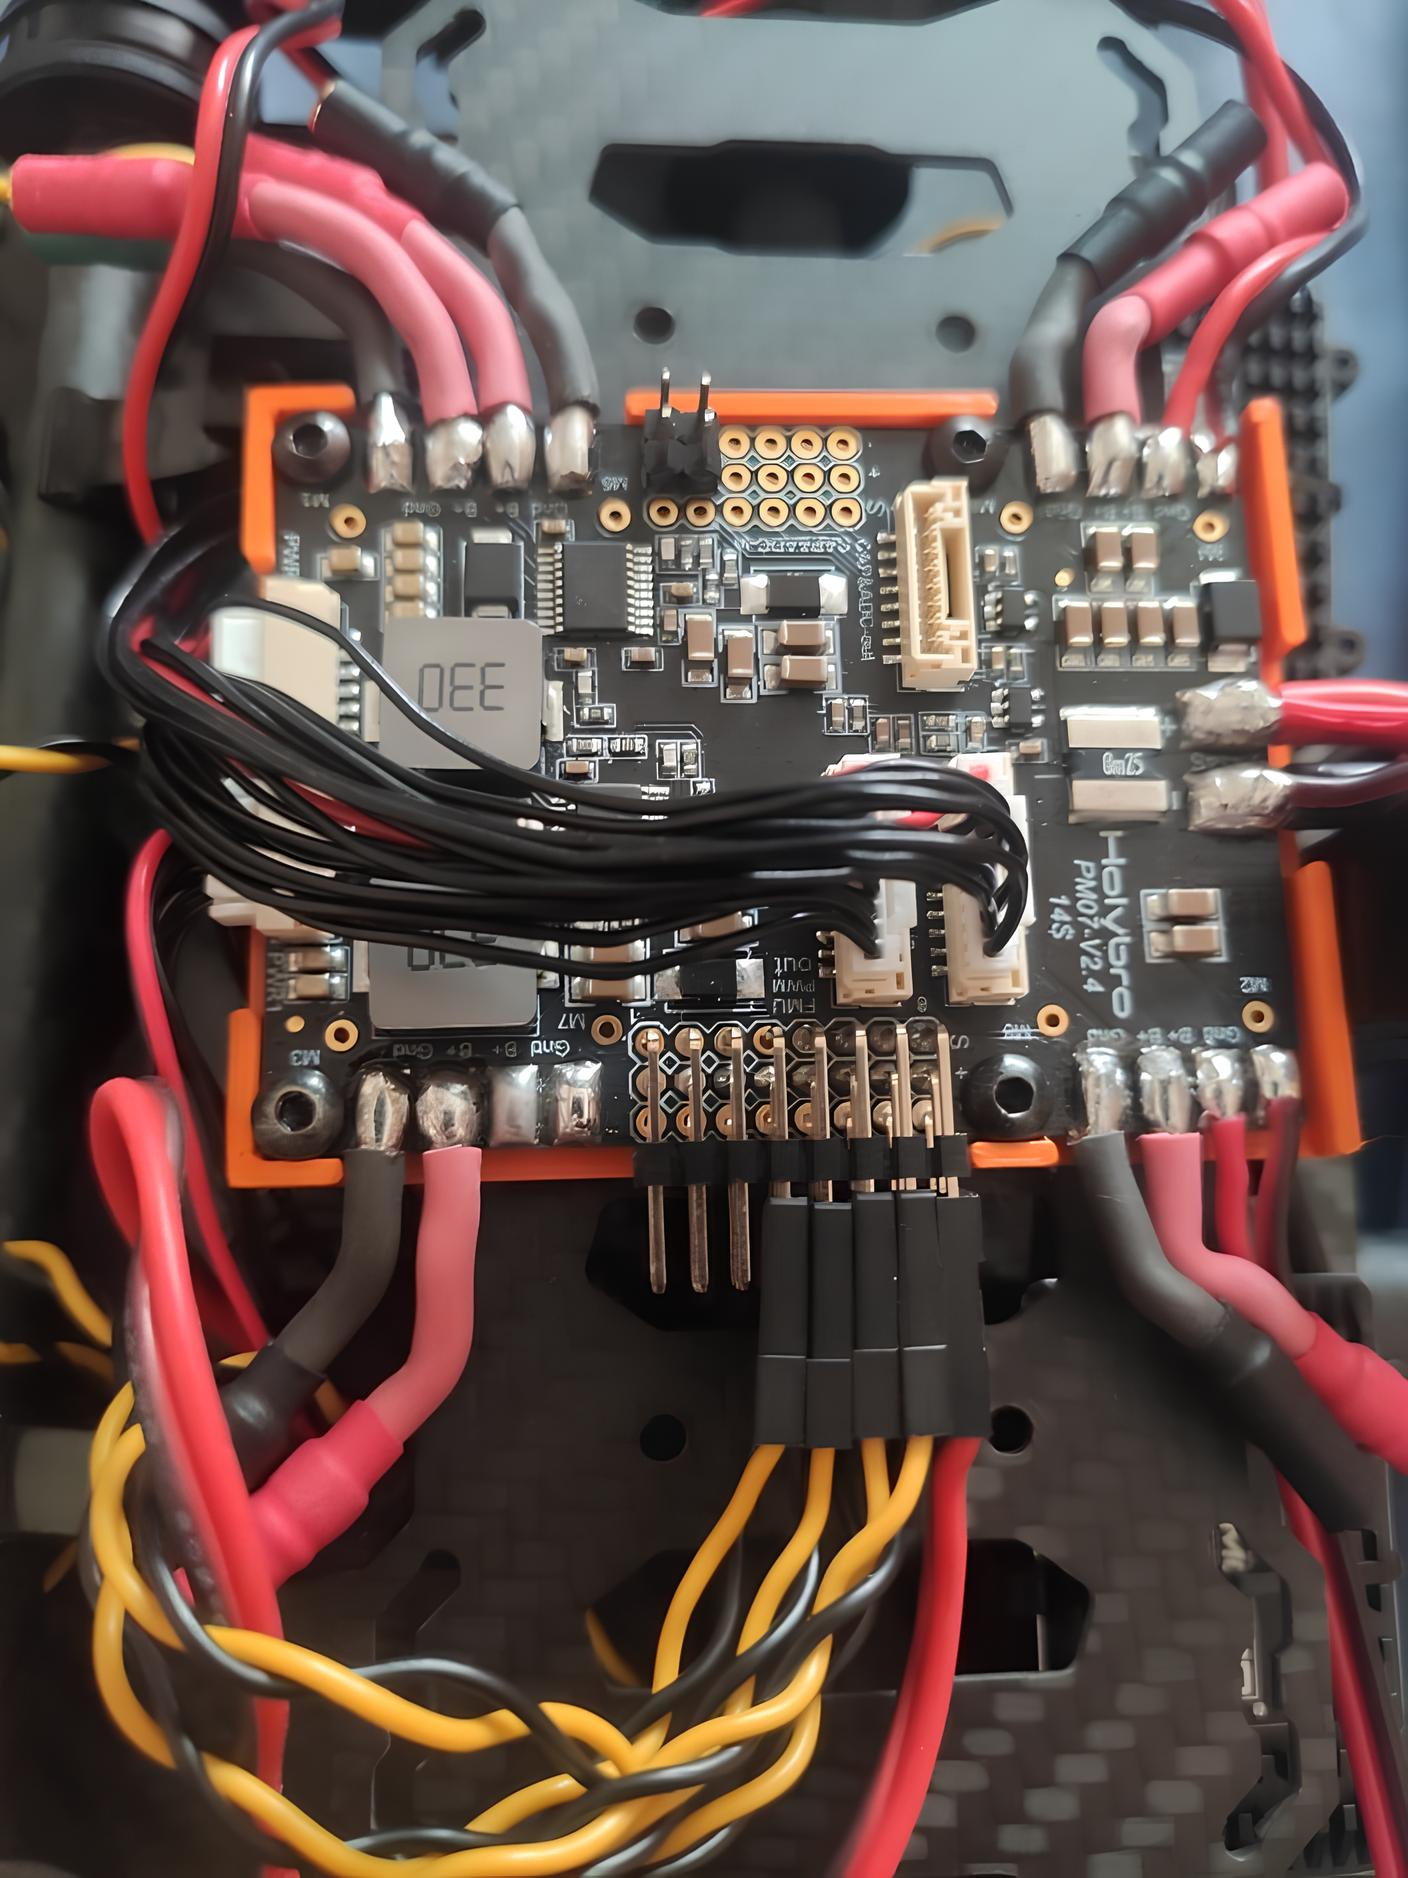
\includegraphics[width=\linewidth]{mid_plate_pdb.jpg}
    \caption{\gls{pdb} attached to the mid plate of the airframe \autocite{developingcosteffectivedrones5g}.}\label{fig:pdb}
  \end{subfigure}
  \hfill
  \begin{subfigure}[t]{0.3\linewidth}
    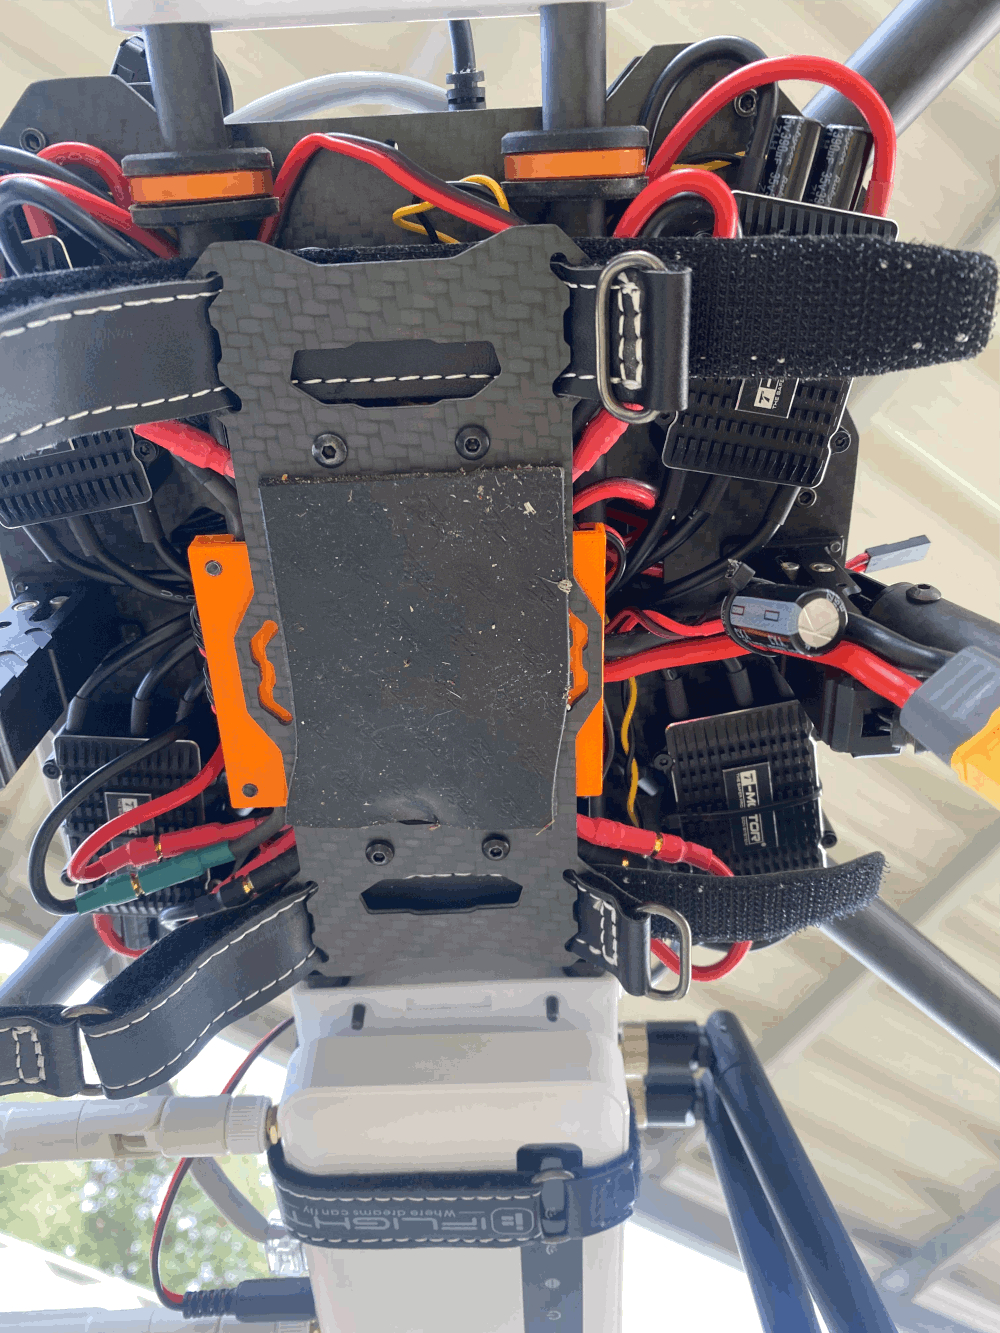
\includegraphics[width=\linewidth]{mid_plate_pdb_mounted.jpg}
    \caption{\gls{pdb} attached to the airframe, orange box in the middle of the airframe.}\label{fig:power_distribution_board_attached_to_airframe}
  \end{subfigure}
  \hfill

  \caption{Power system components attached to the airframe.}\label{fig:power_system_components_attached_to_airframe}
\end{figure}

\subsection{Peripherals}\label{subsec:implementation_peripherals}

The \gls{gps} was attached to the top of the airframe using a custom 3D printed mount, as seen in \cref{fig:gps_attached_to_airframe}. A important note is that the \gls{gps} module must be placed in a location where it has the best reception, as well as where it is not obstructed by other components of the \gls{uav}. It must be place as far as possible from the motors and any carbon fiber components, as they can interfere with the reception of the \gls{gps} module.

For the communication system, the \gls{rf} module was attached to the airframe using the same 3D printed mount as the \gls{gps} module, as seen in \cref{fig:gps_attached_to_airframe}. The \gls{4g} module was attached to the airframe along with the \gls{rf} module and the \gls{gps} module.

The camera was attached to the front of the airframe using a custom 3D printed mount in order to provide the best \gls{fov}, as seen in \cref{fig:camera_attached_to_airframe}. The camera must be placed in a location where it has the best field of view, as well as where it is not obstructed by other components of the \gls{uav}. It must be placed as far as possible from the motors as they can interfere with the camera's \gls{fov}.

Finally, for the on-board computer, it was placed in the middle of the airframe using screws and nuts, as seen in \cref{fig:computer_attached_to_airframe}. It must be placed in a location where air can flow freely to avoid overheating. Depending on the application, the on-board computer can be placed in a different location, as long as it is not obstructed by other components of the \gls{uav}, however, it is recommended to place it in the middle of the airframe to provide the best balance and stability during flight.

\begin{figure}
  \hfill
  \begin{subfigure}[t]{0.3\linewidth}
    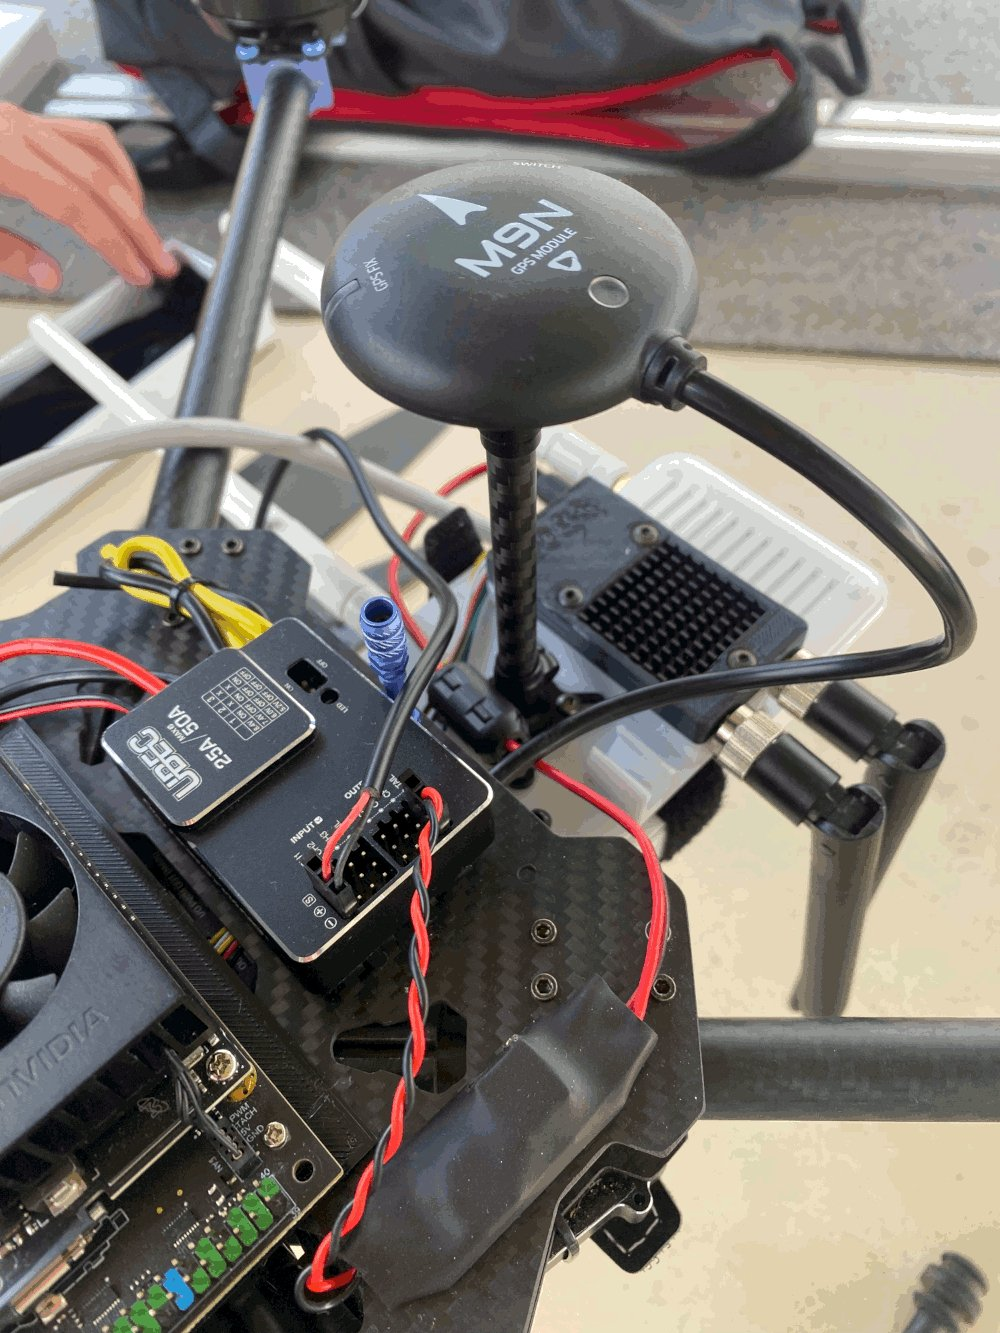
\includegraphics[width=\linewidth]{top_plate_gps.jpg}
    \caption{\gls{gps} module attached to the airframe (circular black module). The \gls{rf} module is the rectangular black module with two antennas behind the \gls{gps} module. The \gls{4g} router is the white module below the \gls{rf} module.}\label{fig:gps_attached_to_airframe}
  \end{subfigure}
  \hfill
  \begin{subfigure}[t]{0.3\linewidth}
    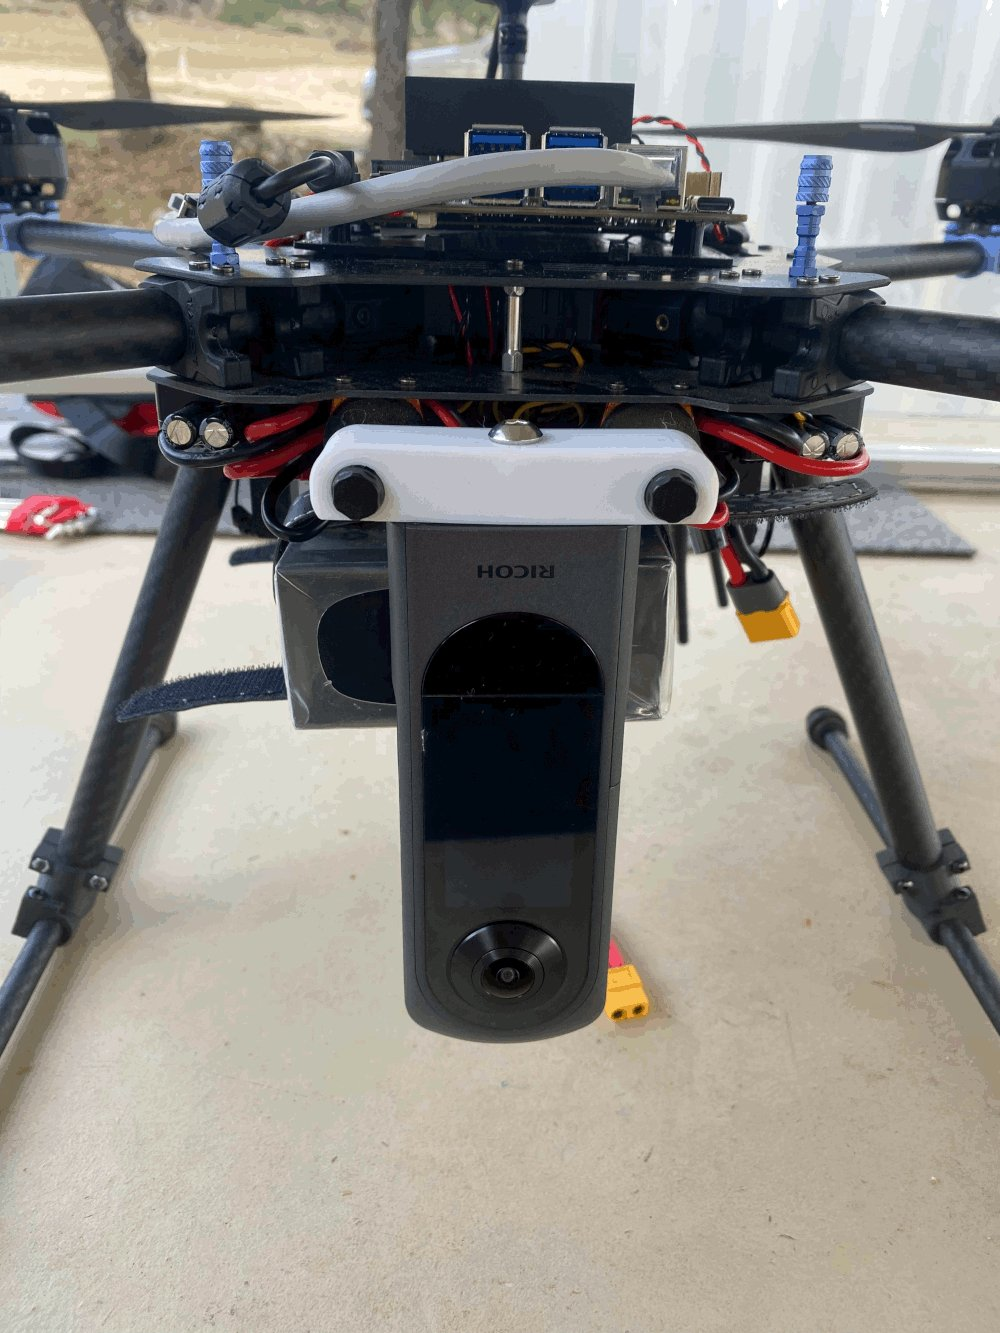
\includegraphics[width=\linewidth]{front_mount_camera.jpg}
    \caption{Camera attached to the airframe using a custom 3D printed white mount.}\label{fig:camera_attached_to_airframe}
  \end{subfigure}
  \hfill
  \begin{subfigure}[t]{0.3\linewidth}
    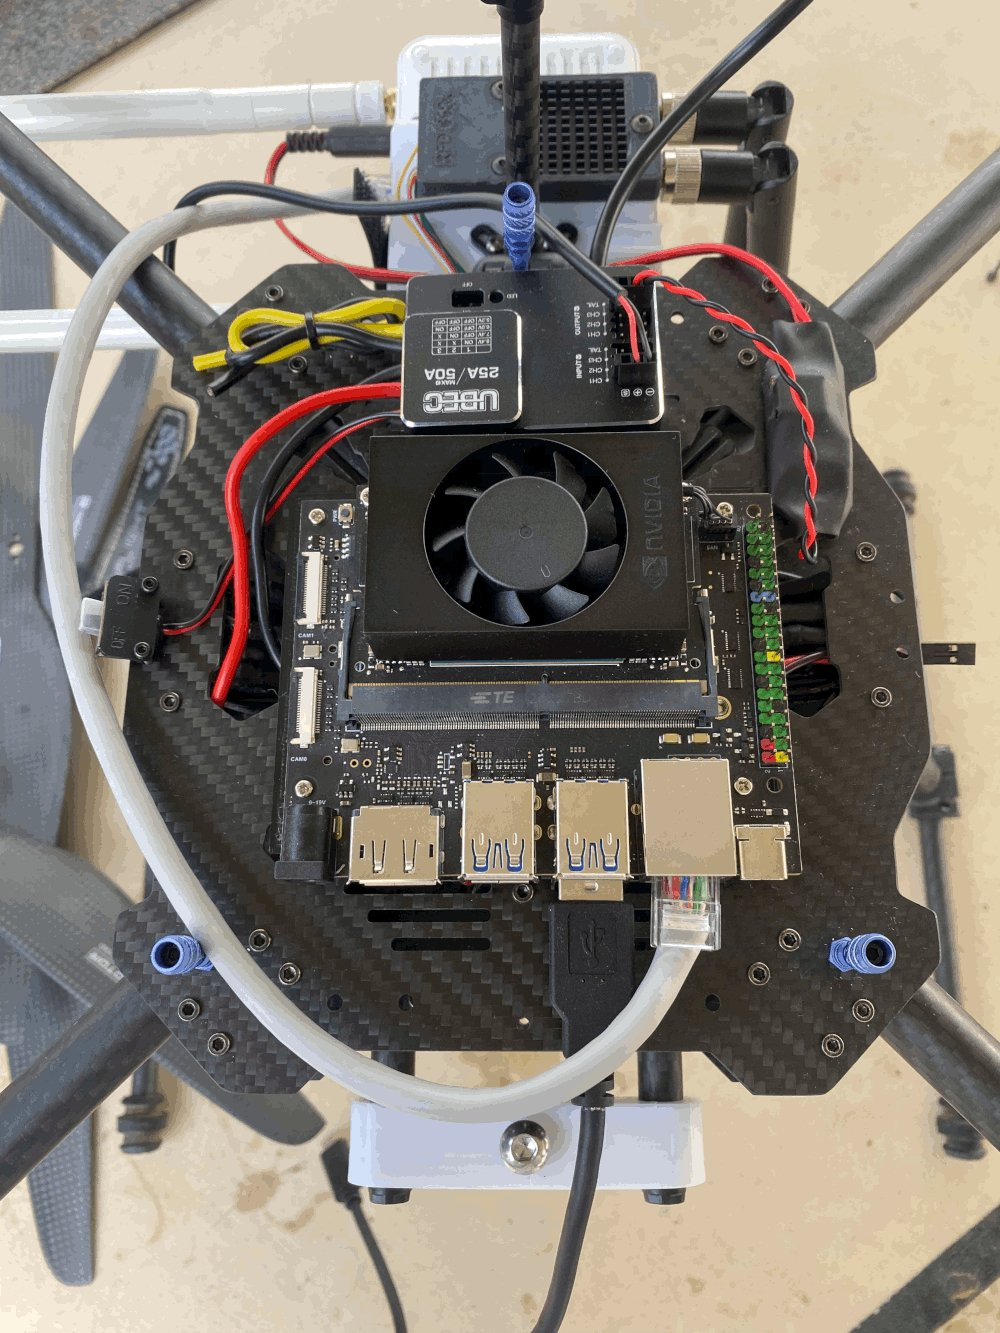
\includegraphics[width=\linewidth]{top_mount_computer.jpg}
    \caption{On the center, the on-board computer. On the top side above the fan, the \gls{gps} module.}\label{fig:computer_attached_to_airframe}
  \end{subfigure}
  \hfill

  \caption{Peripherals attached to the airframe.}\label{fig:peripherals_attached_to_airframe}
\end{figure}

\subsection{Final Assembly}\label{subsec:implementation_final_assembly}

After all the components were attached to the airframe, the final assembly of the \gls{uav} was performed. The final assembly consists of connecting all the components together, as well as configuring the flight controller and the communication system. The final assembly of the \gls{uav} can be seen in \cref{fig:uav_assembled}.

\begin{figure}
  \hfill
  \begin{subfigure}[t]{0.4\linewidth}
    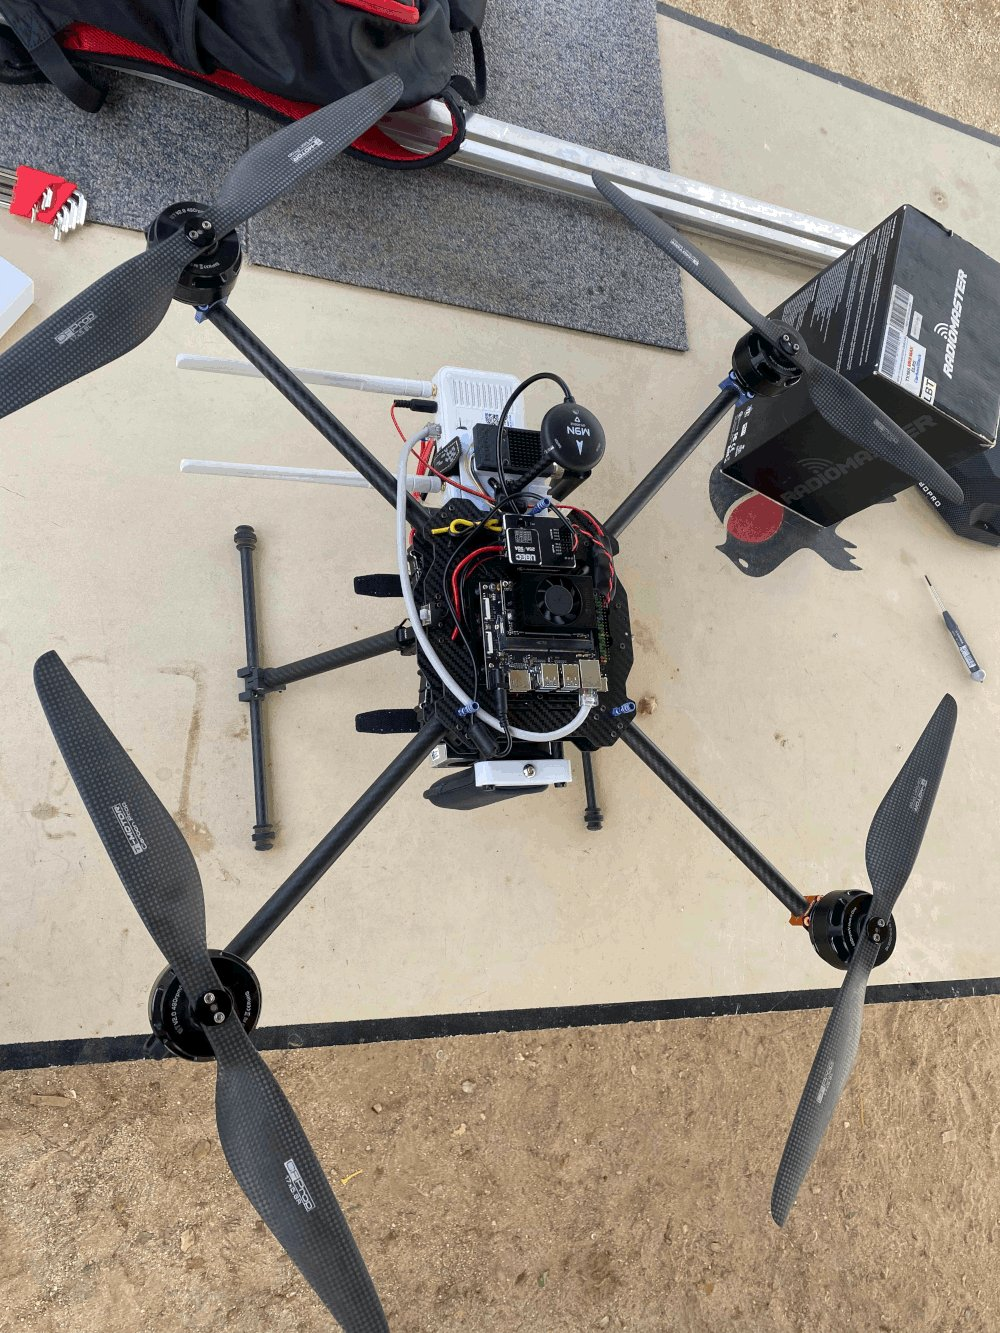
\includegraphics[width=\linewidth]{final_assembly_top.jpg}
    \caption{Top view of the \gls{uav} assembled.}\label{fig:uav_assembled_top}
  \end{subfigure}
  \hfill
  \begin{subfigure}[t]{0.4\linewidth}
    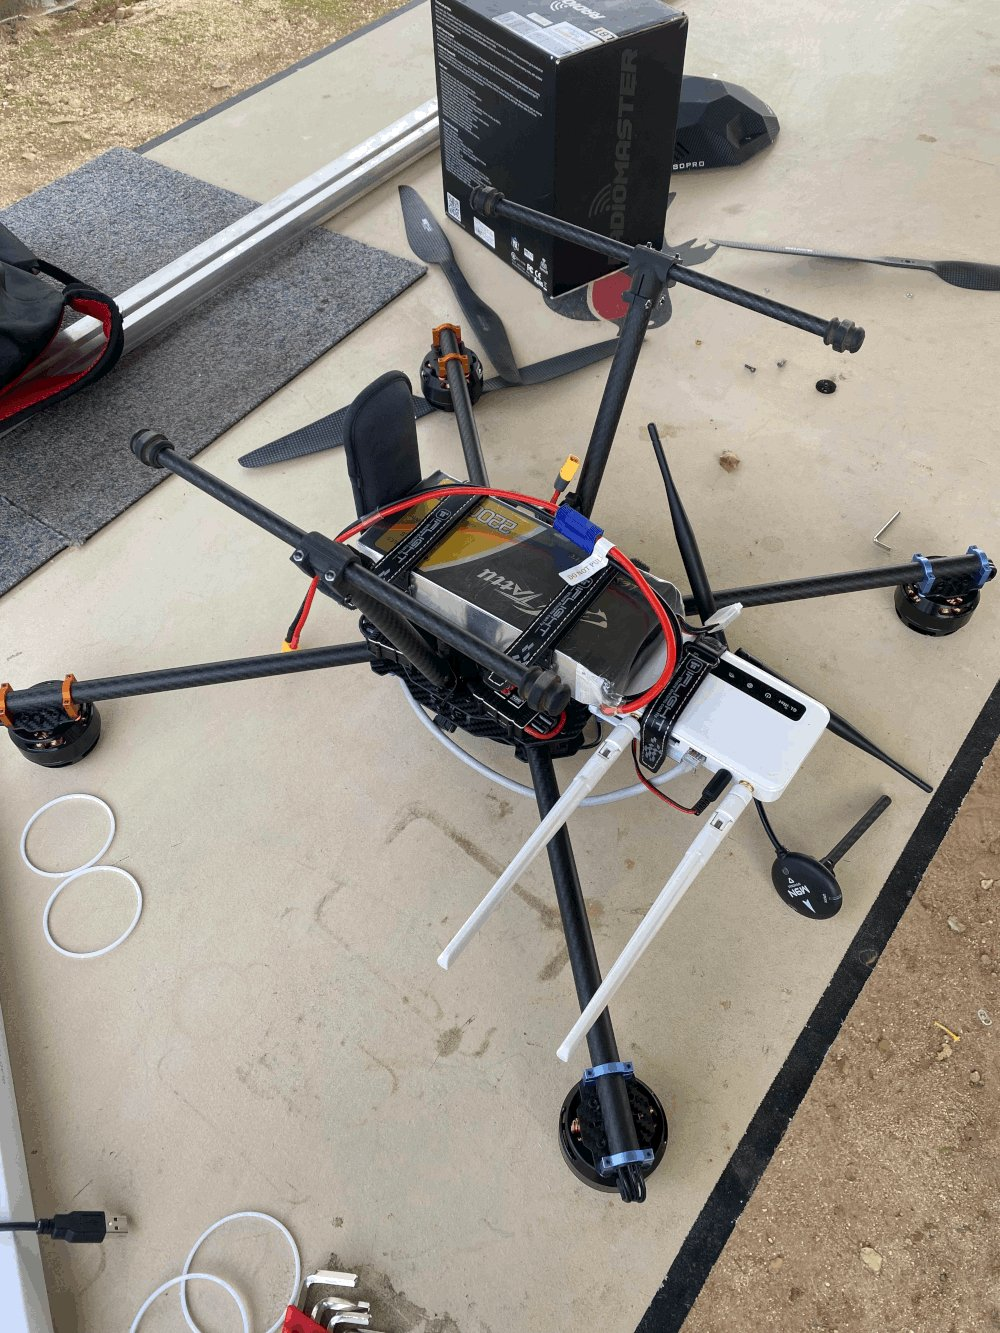
\includegraphics[width=\linewidth]{final_assembly_bottom.jpg}
    \caption{Bottom view of the \gls{uav} assembled.}\label{fig:uav_assembled_bottom}
  \end{subfigure}
  \hfill

  \caption{Final assembly of the \gls{uav}.}\label{fig:uav_assembled}
\end{figure}

\section{Control Station}\label{sec:implementation_control_station}

\section{Communication System}\label{sec:implementation_communication_system}

\section{Reconnaissance Platform}\label{sec:implementation_reconnaissance_platform}

Finally, to implement the reconnaissance platform, three main components are needed: video capture, video processing, and insights generation. The video capture component is responsible for capturing the video feed from the \gls{uav} camera. The video processing component is responsible for processing the video feed to extract relevant information. The insights generation component is responsible for generating insights from the processed video feed. Each different component is implemented separately and then integrated into the reconnaissance platform as a whole.

\subsection{Video Capture}\label{subsec:implementation_video_capture}

In order to capture the video from the Ricoh Theta X 360 Degree Camera \autocite{ricohimagingTHETARicoh}, the camera is connected to the NVIDIA Jetson Orin \autocite{nvidiaNVIDIAJetson} using a \gls{usb} C cable. The camera is configured to stream the video feed to the NVIDIA Jetson Orin using the Ricoh Theta X 360 Degree Camera API \autocite{ricoh360ReferenceRicoh}. In order to be able to capture the video feed from the camera, several libraries are used, such as OpenCV \autocite{githubGitHubOpencvopencv}, GSTThetaUVC \autocite{githubGitHubBuburidergstthetauvc}, LibUVC \autocite{githubGitHub6GIntegration3UC3Mlibuvcthetasample}, and V4L2 \autocite{githubGitHubUmlaeutev4l2loopback}. It is worth mentioning that the libraries used had to be modified to work with the Ricoh Theta X 360 Degree Camera, as it is not officially supported by the libraries. The video feed is captured in real-time and sent to the video processing component for further processing.

\subsection{Video Processing}\label{subsec:implementation_video_processing}

Once the video feed is captured by the Jetson Orin, it is further processed to extract relevant information. The video processing is done using deep learning algorithms to detect and track objects in the environment. The model used for the object detection and tracking is the YOLOv11 \autocite{ultralyticsYOLO11} as it is the defacto standard for object detection and tracking in real-time. It provides the best performance in terms of accuracy and speed, as well as being able to run on the Jetson Orin. The model used was the YOLOv11-medium with a pixel resolution of 640x640 px and an inference time of \SI{56}{\milli\second}. In \cref{fig:drone_yolo_detection}, an example of the video feed captured by the camera can be seen, note a single frame is showcased.

\begin{figure}
	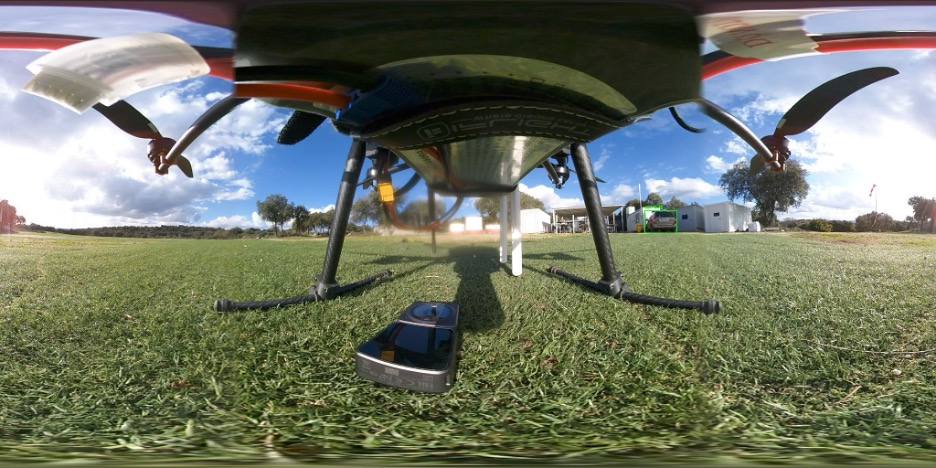
\includegraphics[]{drone_yolo_detection.jpg}
	\caption{Detection example of the video processing with a YOLOv11. The green box  on the middle right side of the image corresponds to the bounding box of the car.}\label{fig:drone_yolo_detection}
\end{figure}

\subsection{Insights Generation}\label{subsec:implementation_insights_generation}

Finally, all the detected and tracked objects are sent to the insights generation component to generate insights for the end-user. In order to process the detected and tracked objects, a web application was developed using the NextJS framework \autocite{nextjsNextjsVercel}. This web application is responsible for displaying the detected and tracked objects in real-time, as well as generating alerts and notifications in case of critical events or failures. The web application is also responsible for managing the different missions of the \glspl{uav} with the objectives and constraints defined by the end-user and also handling the user authentication and authorization.

The web application is divided into three main layers: the presentation layer, the application layer, and the data layer. The application layer is responsible for handling the business logic of the web application, such as the user authentication and authorization, the mission management, the rule management, the detection management, the alert management, and the notification management. The presentation layer is responsible for displaying the information to the end-user. The data layer is responsible for storing the information of the web application.

\subsubsection{Presentation Layer}\label{subsubsec:implementation_presentation_layer}

The presentation layer is developed using the ReactJS framework \autocite{reactReact} for the frontend, Tailwind CSS \autocite{tailwindcssTailwindRapidly} for the styling, and Prisma \autocite{prismaPrismaSimplify} for the database handling. In order to provide a responsive and user-friendly interface, the web application is divided into different components, such as the login component, the dashboard component, the mission component, the drone component. Each component is responsible for displaying the information to the end-user and providing the necessary functionalities to interact with the system. The web application is designed to be easy to use and intuitive, as well as to provide real-time updates and notifications to the end-user. In \cref{fig:web_application}, a screenshot of the web application can be seen.

\begin{figure}
	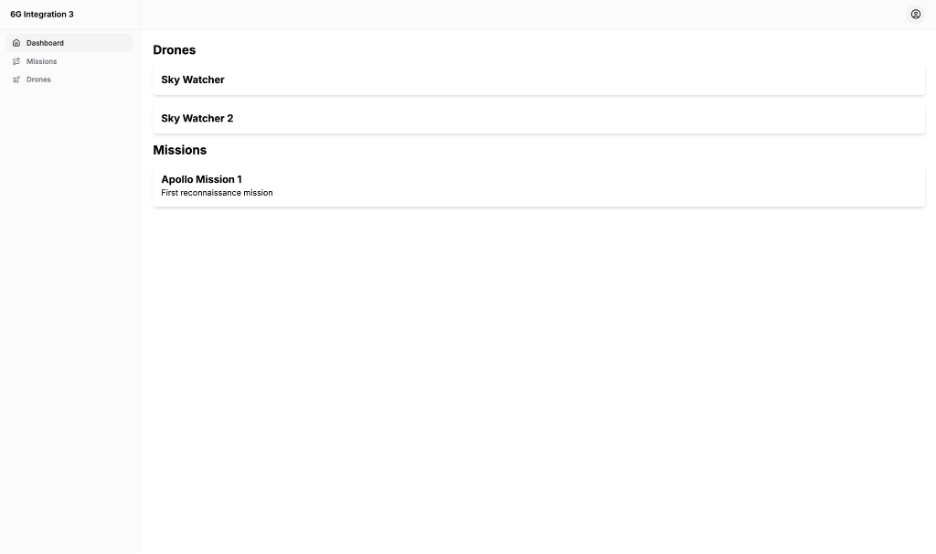
\includegraphics[]{website_showcase.png}
	\caption{Screenshot of the web application showcasing the dashboard.}\label{fig:web_application}
\end{figure}

\subsubsection{Data Layer}\label{subsubsec:implementation_data_layer}

The data layers are divided into two main components: the object storage and the database. The object storage is used to store the video feed captured by the camera, as well as the detected and tracked objects. The object storage used was Amazon S3 \autocite{amazonCloudComputing}, as it provides a reliable and scalable storage solution for the web application.  For the database, a relational database was used to store the information of the web application. As Prisma \autocite{prismaPrismaSimplify} was used for the database handling, the database chosen can be any database supported by Prisma, such as PostgreSQL, MySQL, SQLite. This was chosen to provide flexibility and scalability to the system, as well as to be able to easily switch between databases if needed for different use cases such as testing, development, or production. The schema of the database can be seen in \cref{fig:database_schema}. The schema has six main tables, each one responsible for storing different information:

\begin{itemize}
	\item User: stores the information of the users of the system that can access the web application. It is used for user authentication and authorization purposes.

	\item Drone: stores the information of the drones that are connected to the system. It is used to manage the different drones and their missions. Each drone has a unique identifier, and a specific secret token to authenticate with the system and allow the drone to send the data to the system.

	\item Mission: stores the information of the missions of the drones. It is used to manage the different missions of the drones and group drones together for specific tasks. Each mission can be composed of one or more drones, and each drone can be part of one or more missions. Moreover, users are assigned to missions to have access to the data collected by the drones.

	\item Rule: stores the information of the rules of a specific mission to generate alerts and notifications. It is used to define the objectives and constraints of a mission, such as the specific objects to detect and track, the specific alerts to generate, and the specific notifications to send.

	\item Detection: stores the information of the detected objects in the environment by a drone for a specific mission. It is used to store the detected objects and their properties, such as the class, the confidence, the position, the size, and the orientation.

	\item Alert: stores the information of the alerts generated by the system for a specific mission created by a rule. It is used to store the alerts and their properties, such as the type, the severity, the message, the timestamp, and the status.
\end{itemize}

\begin{figure}
	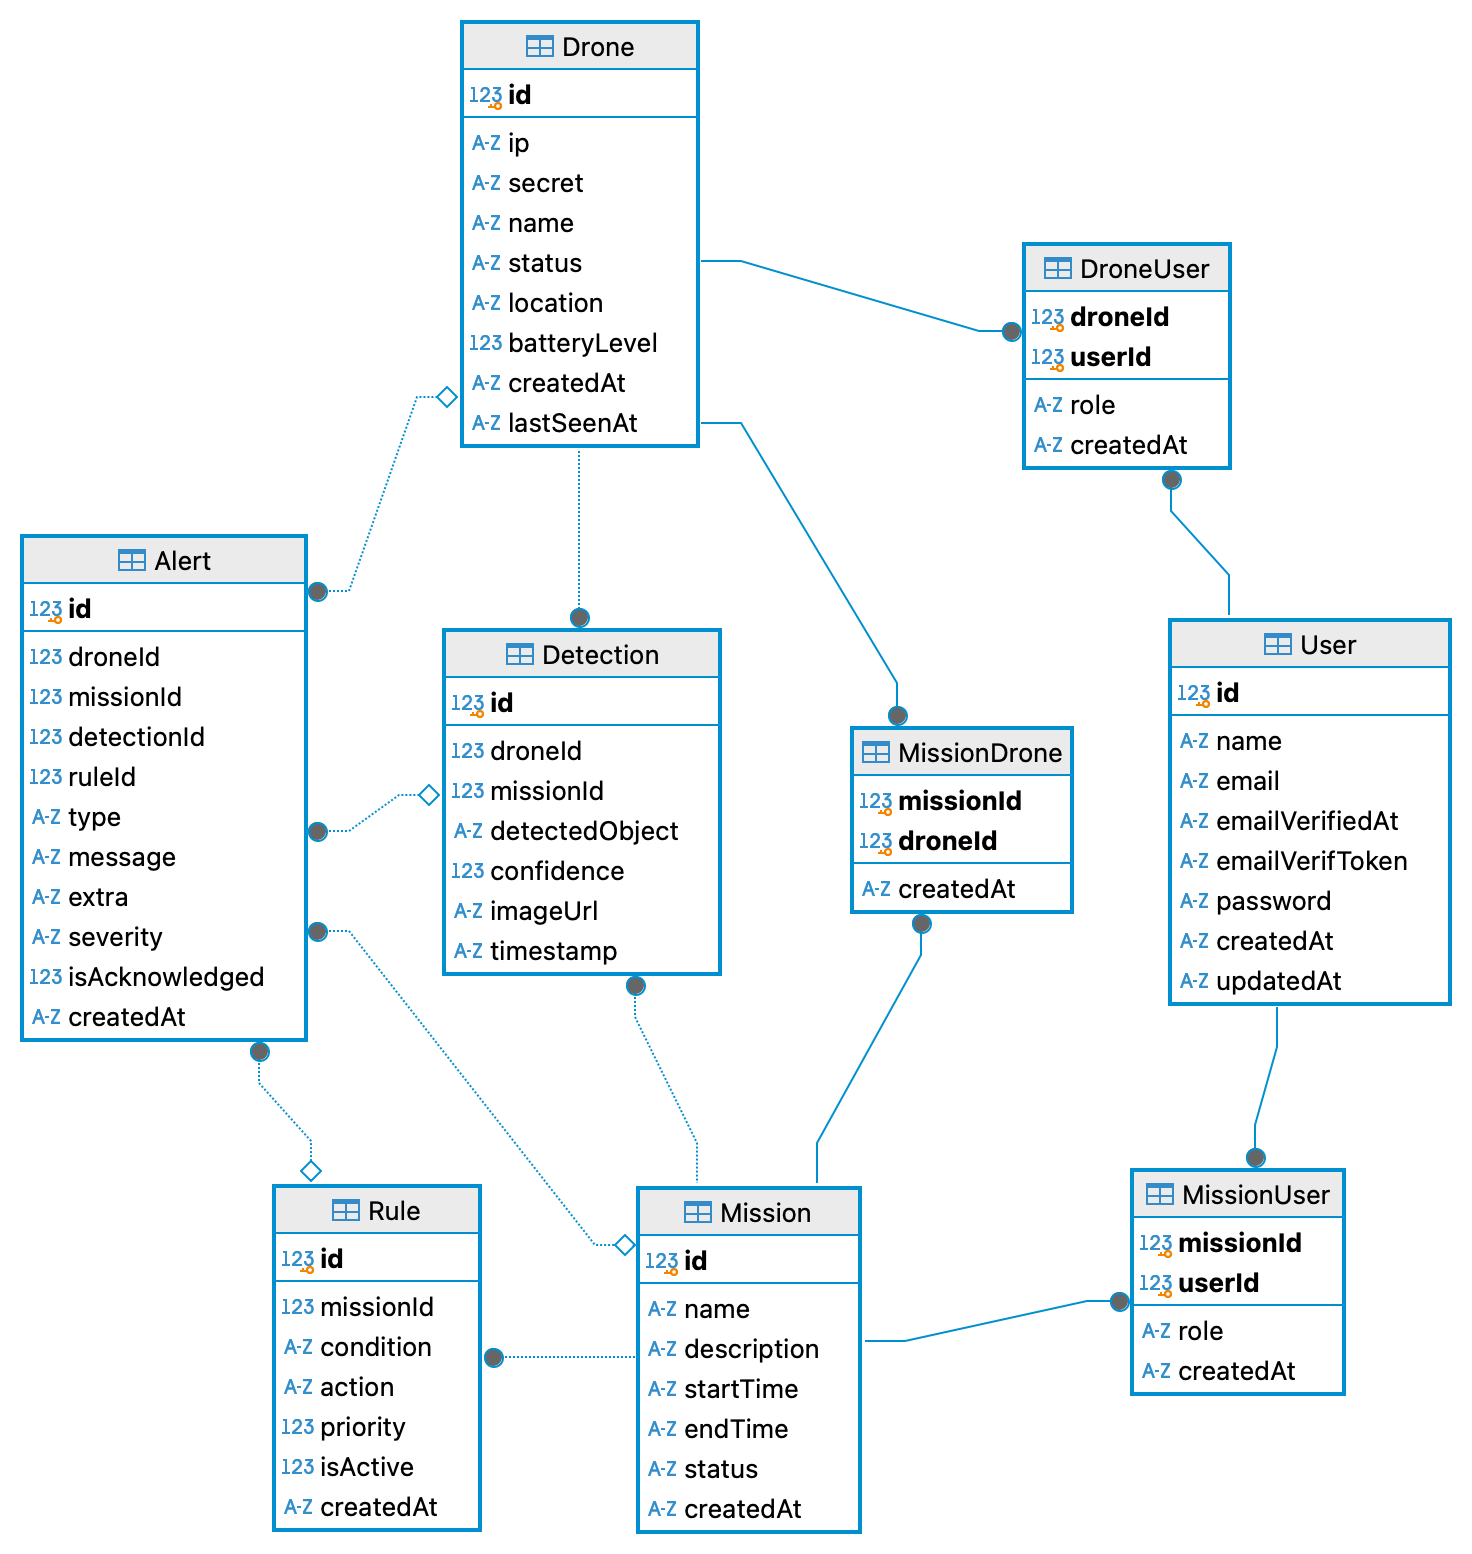
\includegraphics{reconnaissance_platform_database_schema.png}
	\caption{Database schema of the reconnaissance platform.}\label{fig:database_schema}
\end{figure}

\subsubsection{Application Layer}\label{subsubsec:implementation_application_layer}

The application layer forms the core of the web application, handling crucial business logic and system functionalities. This layer is responsible for managing various aspects of the reconnaissance platform, including:

\begin{itemize}
	\item User Authentication and Authorization: Implements secure login mechanisms and controls access to different parts of the system based on user roles and permissions. It is done with email password authentication and verification using the NextAuth.js library \autocite{nextauthNextAuthjsAuthentication}.

	\item Mission Management: Oversees the creation, modification, and execution of drone missions. This includes defining mission parameters, assigning drones, and monitoring mission progress.

	\item Rule Management: Allows users to set up and modify rules for generating alerts and notifications based on specific conditions or events detected during missions.

	\item Detection Management: Processes and organizes the data from detected and tracked objects, making it available for analysis and visualization.

	\item Alert Management: Generates and manages alerts based on predefined rules, ensuring that critical events are promptly communicated to relevant users.

	\item Notification Management: Handles the distribution of notifications to users through various channels, keeping them informed about mission status, alerts, and system updates.
\end{itemize}

The application layer serves as the intermediary between the presentation layer and the data layer, ensuring efficient data flow and processing. It implements the business logic that interprets user actions from the presentation layer, interacts with the data layer to retrieve or store information, and prepares the data for display in the user interface.

\subsubsection{LLM Integration}\label{subsubsec:implementation_llm_integration}

Moreover, the detected and tracked objects are further processed through an \gls{llm} integration, in this case Llama 3.2 11b Vision \autocite{llama3.211bvision}, using the Groq \glsentryshort{api} to extract additional contextual information and insights. This integration enhances the system's analytical capabilities by providing detailed descriptions, identifying potential relationships between detected objects, and generating natural language summaries of the surveillance data.

The \gls{llm} component receives the object detection data from the server with a specific prompt that the server operator wants to send and processes it to provide comprehensive analysis that includes object classification details, behavioral patterns, and potential security implications. This additional layer of intelligence helps operators make more informed decisions by providing context-rich information about the detected objects in real-time. The results from the \gls{llm} analysis are stored in the database and made available through the web interface, where they can be accessed alongside the original detection data and visual feeds.

In \cref{fig:llm_detection}, an example of the \gls{llm} detection results for a person can be seen.

\begin{figure}
	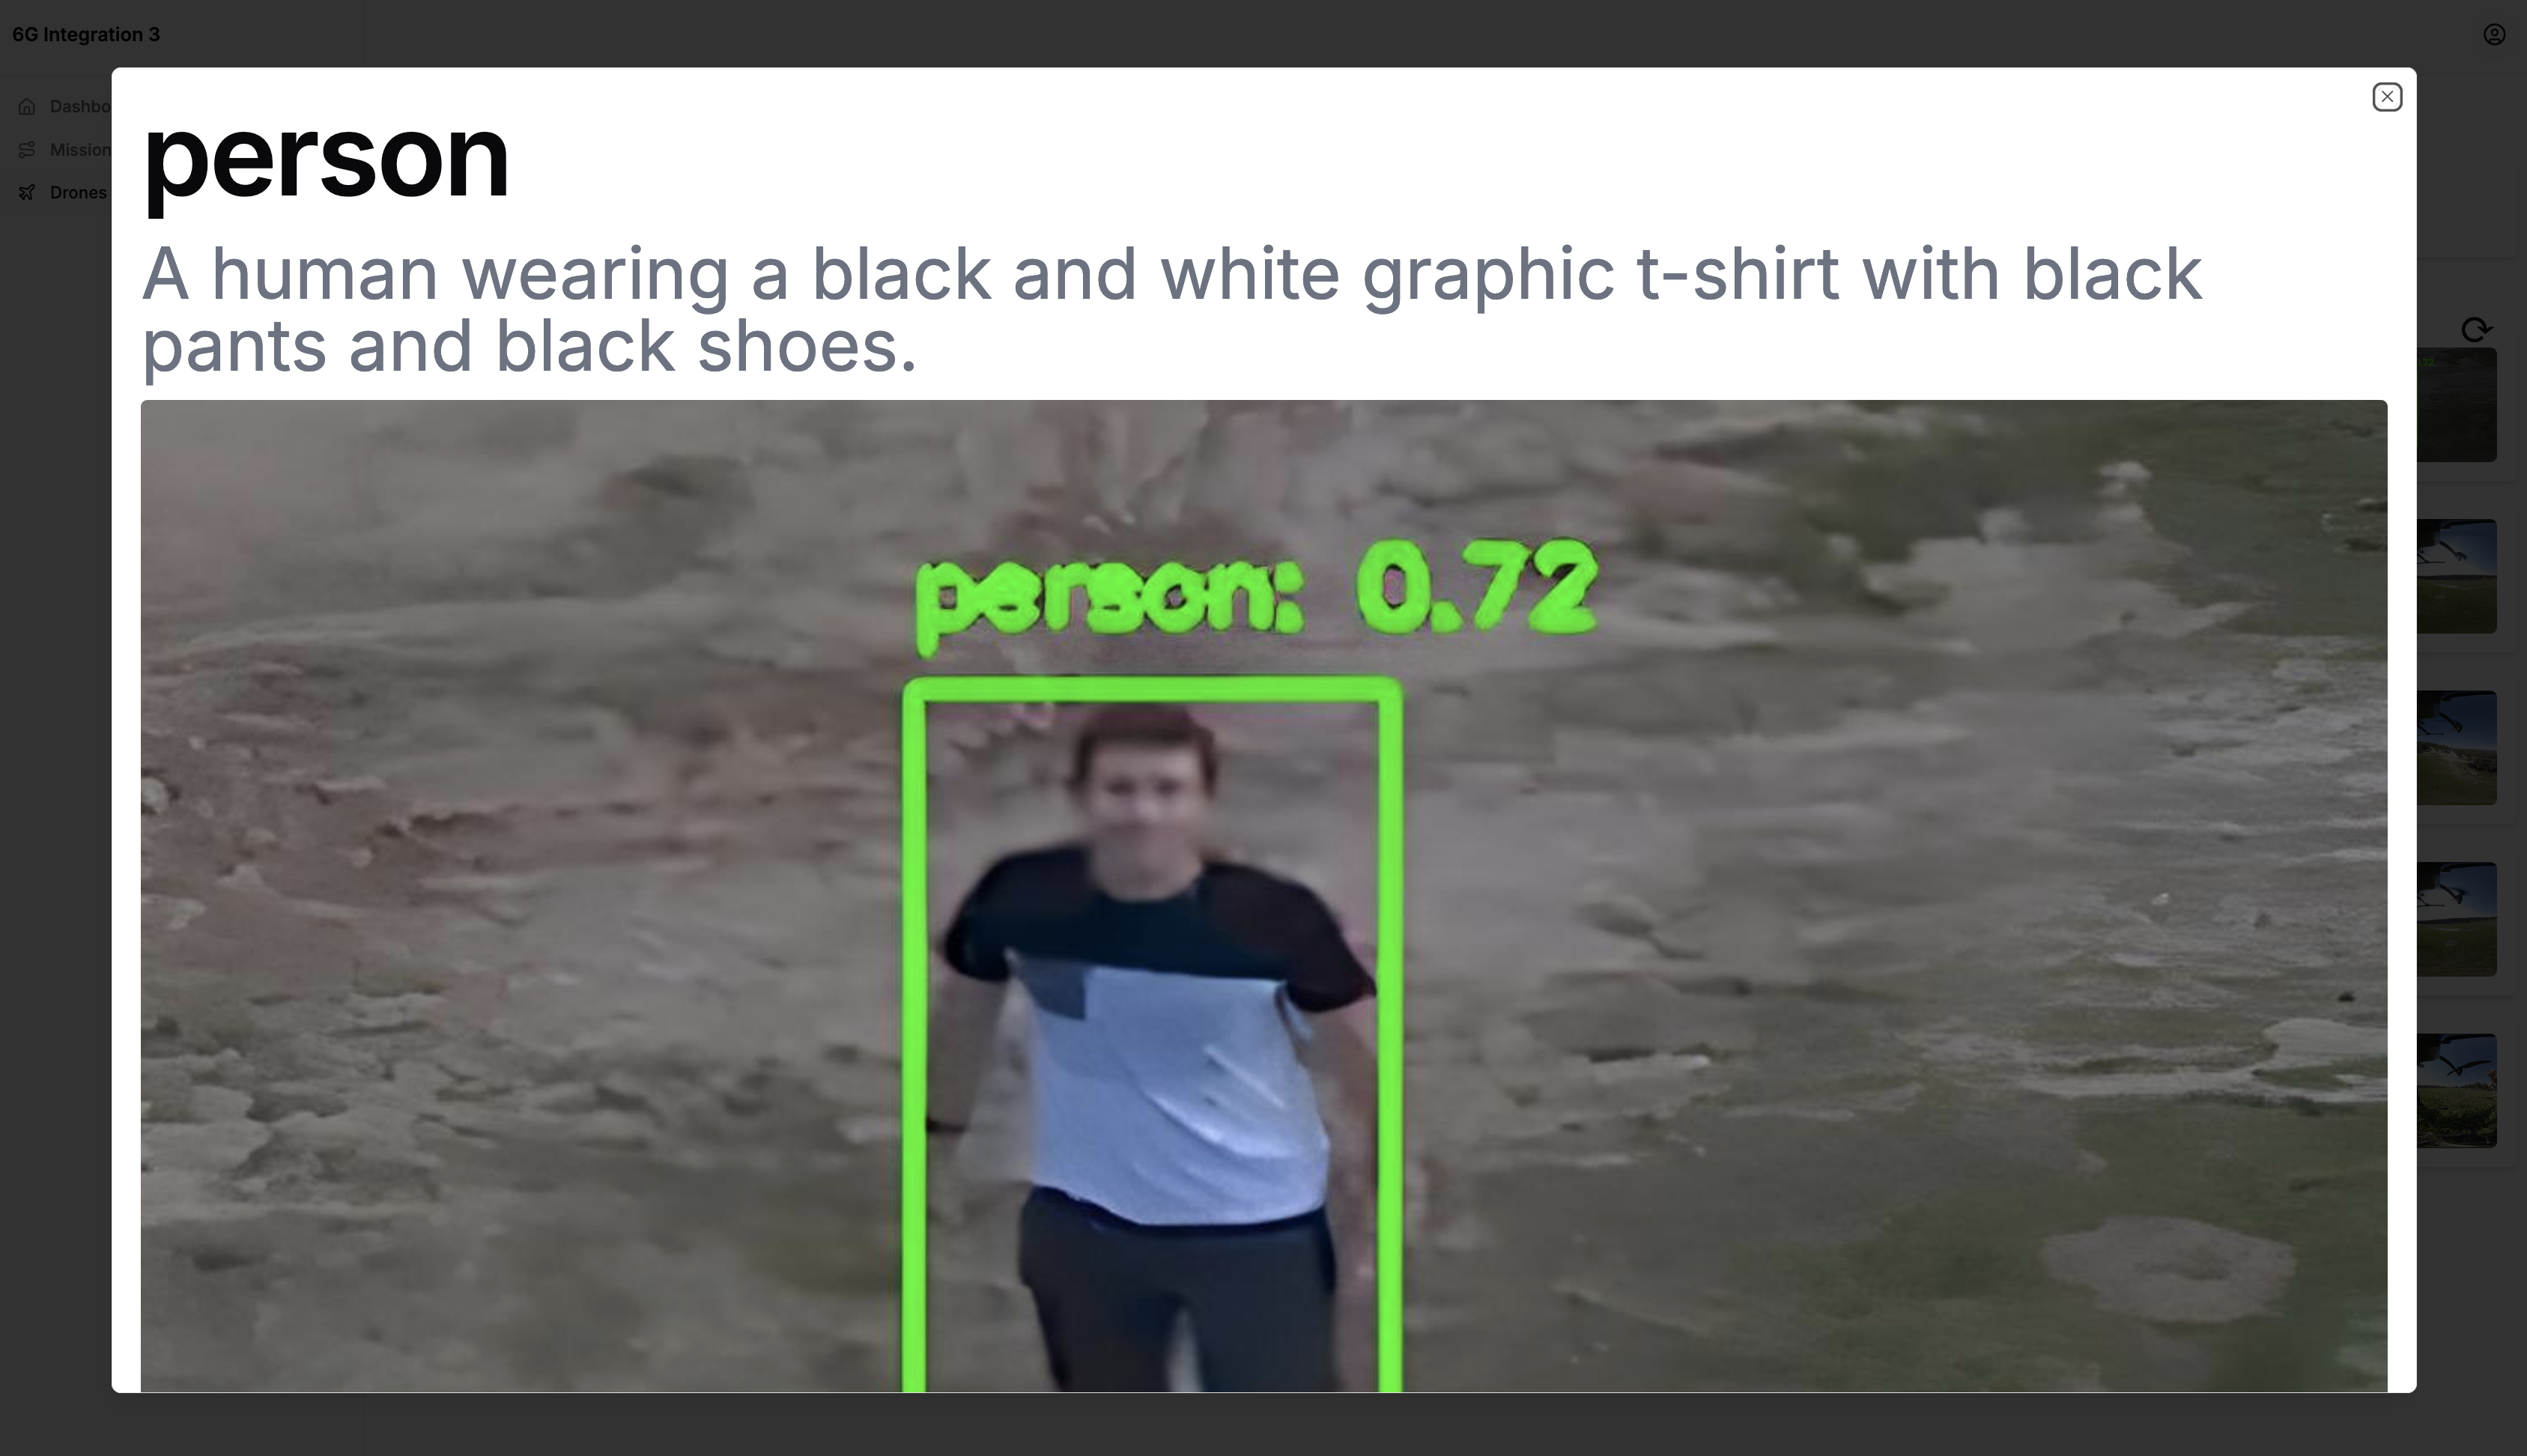
\includegraphics{llm_detection.png}
	\caption{Example of the LLM detection results for a detected object. In this case, the LLM correctly identified the clothes that the person is wearing as the prompt to the image was ``What is the person wearing?''.}\label{fig:llm_detection}
\end{figure}

\subsection{Integration}\label{subsec:implementation_integration}

Finally, all the different components are integrated into the reconnaissance platform to provide a complete processing pipeline to be able to detect the different objects. In \cref{fig:architecture_reconnaissance_platform}, the complete architecture and pipeline can be seen and consists of several interconnected components:

\begin{itemize}
	\item \textbf{Drone Component:} Contains two primary elements:
	      \begin{itemize}
		      \item 360-degree camera for capturing omnidirectional video feed
		      \item Object detection system running directly on the drone for initial processing
	      \end{itemize}
	\item \textbf{VPN Tunnel:} Provides a secure communication channel between the drone and the server infrastructure, ensuring encrypted data transmission.
	\item \textbf{Server Infrastructure:} Comprises two main processing units:
	      \begin{itemize}
		      \item Object Detection module for secondary verification and processing
		      \item Alert system for generating notifications based on detected events
	      \end{itemize}
	\item \textbf{LLM Integration:} The final component in the pipeline that:
	      \begin{itemize}
		      \item Processes detected objects through advanced language models
		      \item Generates contextual insights and natural language descriptions
		      \item Provides enhanced analytical capabilities for operators
	      \end{itemize}
\end{itemize}

The data flow in this architecture follows a sequential pattern where the video feed from the 360-degree camera is first processed locally on the drone for initial object detection. This data is then transmitted through a secure VPN tunnel to the server infrastructure, where it undergoes additional processing and verification. The server component handles both the object detection confirmation and alert generation based on predefined rules and conditions. Finally, the processed data is passed to the LLM integration component, which provides advanced analysis and insights generation for the end-users through the web interface.

This architecture ensures robust security through the VPN tunnel while maintaining efficient data processing and real-time analysis capabilities. The modular design allows for easy scaling and maintenance of individual components without affecting the overall system functionality.

\begin{figure}
	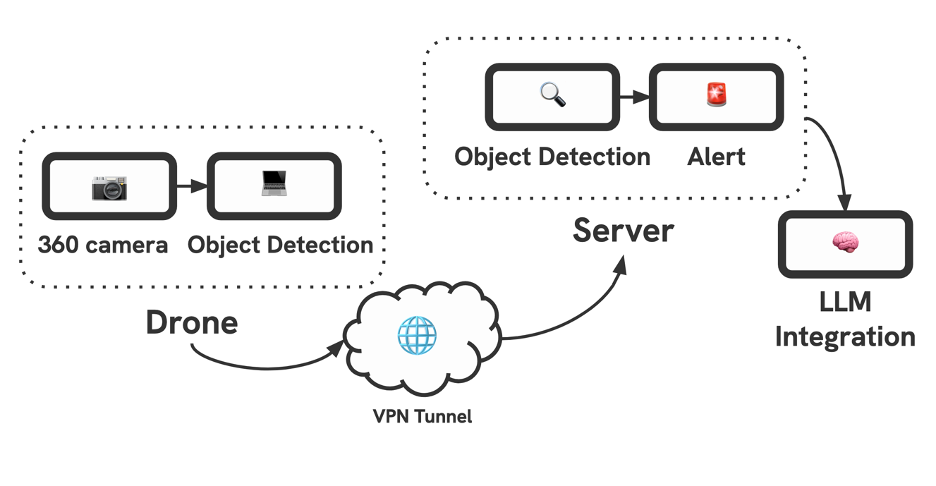
\includegraphics{architecture_reconnaissance_platform.png}
	\caption{Architecture of the reconnaissance platform.} \label{fig:architecture_reconnaissance_platform}
\end{figure}



% Local Variables:
% jinx-local-words: "uav"
% End:

\chapter{Testing}
\label{ch:testing}

\todo{write this chapter}


\part{Results}

\part{Conclusions}

\chapter{Conclusions}\label{ch:conclusions}

This thesis presents a comprehensive approach to developing and implementing an autonomous drone system for \gls{ntn} in remote areas. The project successfully achieved its objectives of creating a modular, cost-effective, and open-source solution that can be easily adapted for various reconnaissance tasks. The implemented system demonstrates the potential of integrating \glspl{uav} with advanced communication technologies and artificial intelligence to enhance connectivity and data collection in challenging environments.

The designed \gls{uav} platform, equipped with a 360-degree camera and onboard processing capabilities, proved capable of autonomous flight and real-time object detection. The integration of a secure communication system, combining \gls{rf} and \gls{4g} technologies, enabled reliable data transmission between the drone and the control station. Furthermore, the development of a sophisticated reconnaissance platform, leveraging deep learning algorithms and \glspl{llm}, showcased the system's ability to provide valuable insights from collected data.

The project's modular approach and use of commercially available components make it accessible for other researchers and organizations to replicate and build upon. This aligns well with the goal of fostering new research in the field of non-terrestrial networks and low-altitude drone-based systems. The successful implementation and testing of the system in a controlled environment demonstrated its potential for applications in humanitarian aid, environmental monitoring, and disaster response.

While some challenges were encountered during the development process, particularly in component selection and system integration, these were ultimately overcome through iterative design and testing. The final system met all specified requirements, including flight duration, autonomous operation, and real-time data processing capabilities.

In conclusion, this thesis contributes a valuable proof-of-concept for autonomous drone systems in non-terrestrial networks, paving the way for future advancements in this field. The developed platform offers a flexible foundation for further research and practical applications in remote area connectivity and reconnaissance.

\chapter{Future works}\label{ch:future_work}

\todo{write this chapter}

\chapter{Socio-economic environment}\label{ch:socio_economic_environment}

The widespread adoption of \glspl{uav} is transforming society and the economy, offering significant benefits while also presenting challenges. This chapter examines the socio-economic factors influencing the deployment of autonomous drones, particularly in \glspl{ntn} for remote areas. It explores the potential advantages, obstacles, and financial implications of integrating this technology across industries.

\section{Social Impact}\label{sec:social_impact}

Autonomous \glspl{uav} have gained popularity due to their versatility and efficiency, revolutionizing fields like agriculture, construction, and public safety. Their ability to perform complex tasks quickly can greatly enhance societal well-being. For example, \glspl{uav} equipped with thermal cameras improve emergency response by locating individuals in burning buildings, while high-resolution cameras can monitor large events. The project demonstrated how \glspl{uav} can provide real-time reconnaissance, aiding first responders and improving public safety.

In remote regions, autonomous \glspl{uav} facilitate connectivity by delivering essential supplies such as medicine and food. This capability not only improves the quality of life but also bridges the digital divide by providing internet access to underserved communities, thereby enhancing educational and informational resources.

However, privacy and security remain concerns. The extensive data collection by \glspl{uav} raises issues of surveillance, while the potential for misuse, such as spying or attacks, underscores the need for clear regulations and ethical guidelines, see \cref{ch:regulatory_framework}.

\section{Economic Impact}\label{sec:economic_impact}

The economic benefits of adopting autonomous \glspl{uav} are substantial, with the potential to boost productivity and drive innovation. In agriculture, \glspl{uav} enable precision farming through crop monitoring, pest detection, and optimized irrigation, helping farmers improve yields and reduce costs. The construction industry also benefits, as \glspl{uav} offer efficient infrastructure inspections, reducing manual labor and associated risks.

Despite these advantages, the costs of adopting \glspl{uav} (e.g., purchase, training, maintenance, and insurance) remain significant barriers for small companies and groups. Moreover, the need for skilled operators and the risk of accidents or malfunctions can increase operational expenses which is specially challenging for research groups in \glspl{ntn}.

\section{Environmental Impact}\label{sec:environmental_impact}

Autonomous \glspl{uav} can positively impact the environment by reducing fossil fuel usage. Their electric motors are more energy-efficient and produce fewer emissions than traditional vehicles, contributing to lower air pollution and greenhouse gas levels.

Nonetheless, the environmental costs of manufacturing and disposing of \glspl{uav} must be considered. The production of lightweight materials like carbon fiber is energy-intensive, and lithium-ion batteries pose recycling challenges. Sustainable design practices are necessary to mitigate these effects.

\section{Budget Analysis}\label{sec:budget_analysis}

As previously mentioned, the cost of adopting autonomous drones is a significant hurdle. This section breaks down the expenses associated with purchasing and operating drones, categorized into manufacturing, operating, and additional costs. The analysis includes a detailed assessment of hardware components, maintenance, insurance, and other relevant expenses.

Tables \cref{tab:manufacturing_costs_uav}, \cref{tab:manufacturing_costs_reconnaissance_platform}, \cref{tab:operating_costs}, and \cref{tab:other_costs} provide comprehensive cost breakdowns. The total cost, encompassing all categories, offers a clear picture of the financial investment needed for adopting drones in \glspl{ntn} applications. For this project, the total cost amounts to \todo{total cost}, which includes the necessary hardware, software, and operational expenses. However, it does not account for human-related costs, such as training and salaries, which are essential for long-term sustainability.

In conclusion, while autonomous drones hold significant promise for remote areas and various industries, careful consideration of social, economic, and environmental factors is essential. Addressing these challenges with appropriate regulations and sustainable practices will maximize their potential benefits.

\begin{table}[H]
  \begin{tabular}{ l l r r }
    \toprule
    \textbf{Item} & \textbf{Model} & \textbf{Quantity} & \textbf{Cost (\euro)} \\
    \midrule
    Airframe & Tarot XS690 \autocite{rcinnovationsQuadPlegable} & 1 & 199 \\
    Motors & Tmotor U7 V2 420KV \autocite{rcinnovationsTmotor420KV} & 4 & 520 \\
    \gls{esc} & Tmotor FLAME 100A LV 600Hz \autocite{rcinnovationsVariadorTmotor} & 4 & 360 \\
    Propellers & Tmotor 17$\times$5.8 V2 \autocite{rcinnovationsTmotor17x58} & 2 & 144 \\
    Flight Controller & Holybro Pixhawk 6C \autocite{rcinnovationsPixhawkCarcasa} & 1 & 207 \\
    Battery & TATTU 22000mAh 4S 14.8V 30C \autocite{rcinnovationsComprarBatera}  & 1 & 270 \\
    \gls{pdb} & HobbyWing 25A HV UBEC \autocite{rcinnovationsHobbyWingUbec} & 1 & 58 \\
    \gls{gps} & Holybro M9N GPS GNSS \autocite{rcinnovationsHolybroGNSS} & 1 & 70 \\
    Radiocontroller & RadioMaster TX16S \autocite{rcinnovationsRadioMasterTX16S} & 1 & 200 \\
    \gls{rf} Module & RFD868 TXMOD V2 868Mhz 1W \autocite{rcinnovationsComprarMdulos} & 1 & 423 \\
    Miscellaneous & Screws, Nuts, Wires, etc. &~--~& 100 \\
    \midrule
    \textbf{Total} & & & 2551 \\
    \bottomrule
  \end{tabular}
  \caption{Manufacturing costs for the \gls{uav}.}\label{tab:manufacturing_costs_uav}
\end{table}

\begin{table}[H]
  \begin{tabular}{ l l l r }
    \toprule
    \textbf{Item} & \textbf{Model} & \textbf{Quantity} & \textbf{Cost (\euro)} \\
    \midrule
    On-board Computer & NVIDIA Jetson Orin \autocite{nvidiaNVIDIAJetson} & 1 & 831 \\
    Camera & Ricoh Theta X 360 Degree Camera \autocite{ricohimagingTHETARicoh} & 1 & 800 \\
    Router & \todo{add ref to where we bought} & 1 &  \\
    4G SIM Card & Orange Prepaid SIM Card (1 month) & 1 & 10 \\
    Server & Amazon Web Services (1 month) & 1 & 10 \\
    \midrule
    \textbf{Total} & & & 1651 \\
    \bottomrule
  \end{tabular}
  \caption{Manufacturing costs for the reconnaissance platform} \label{tab:manufacturing_costs_reconnaissance_platform}
\end{table}

\begin{table}[H]
    \begin{tabular}{ l l r }
        \toprule
        \textbf{Item} & \textbf{Description} & \textbf{Cost (\euro)} \\
        \midrule
        Insurance & Liability Insurance for Pilots & 50 \\
        Flying Field & Flying Club Membership (1 year) & 350 \\
        Licensing & Drone Pilot License (1 year) & 0 \\
        Software & ArduPilot Software License (1 year) & 0 \\
        Maintenance & Spare Parts & 50 \\
        \midrule
        \textbf{Total} & & 450 \\
        \bottomrule
    \end{tabular}
    \caption{Operating costs.}\label{tab:operating_costs}
\end{table}

\begin{table}[H]
    \begin{tabular}{ l l r r }
        \toprule
        \textbf{Item} & \textbf{Model} & \textbf{Quantity} & \textbf{Cost (\euro)} \\
        \midrule
        Battery Charger & ISDT K4 Dual Charger \autocite{rcinnovationsISDTCargador} & 1 & 200 \\
        Lipo Bags & Lipo Safe Bags (Large) \autocite{rcinnovationsBolsaProtectora} & 1 & 13 \\
        Tools & Screwdriver Set, Pliers, etc. &~--~& 50 \\
        Solders & Soldering Iron, Solder, etc. &~--~& 200 \\
        3D Printer & Bamboo P1S \autocite{bambulabBambuPrinter} & 1 & 1015 \\
        3D Filament & PLA Filament (1kg) & 1 & 30 \\
        \midrule
        \textbf{Total} & & & 1508 \\
        \bottomrule
    \end{tabular}
    \caption{Other costs.}\label{tab:other_costs}
\end{table}

% Local Variables:
% jinx-local-words: "Holybro Pixhawk Tmotor ntn nvidiaNVIDIAJetson pdb rcinnovationsComprarBatera rcinnovationsComprarMdulos rcinnovationsHobbyWingUbec rcinnovationsHolybroGNSS rcinnovationsPixhawkCarcasa rcinnovationsQuadPlegable rcinnovationsVariadorTmotor rf ricohimagingTHETARicoh uav"
% End:


\blankpage%
\printbibliography%

\end{document}
